\documentclass[twoside]{book}

% Packages required by doxygen
\usepackage{fixltx2e}
\usepackage{calc}
\usepackage{doxygen}
\usepackage[export]{adjustbox} % also loads graphicx
\usepackage{graphicx}
\usepackage[utf8]{inputenc}
\usepackage{makeidx}
\usepackage{multicol}
\usepackage{multirow}
\PassOptionsToPackage{warn}{textcomp}
\usepackage{textcomp}
\usepackage[nointegrals]{wasysym}
\usepackage[table]{xcolor}

% Font selection
\usepackage[T1]{fontenc}
\usepackage[scaled=.90]{helvet}
\usepackage{courier}
\usepackage{amssymb}
\usepackage{sectsty}
\renewcommand{\familydefault}{\sfdefault}
\allsectionsfont{%
  \fontseries{bc}\selectfont%
  \color{darkgray}%
}
\renewcommand{\DoxyLabelFont}{%
  \fontseries{bc}\selectfont%
  \color{darkgray}%
}
\newcommand{\+}{\discretionary{\mbox{\scriptsize$\hookleftarrow$}}{}{}}

% Page & text layout
\usepackage{geometry}
\geometry{%
  a4paper,%
  top=2.5cm,%
  bottom=2.5cm,%
  left=2.5cm,%
  right=2.5cm%
}
\tolerance=750
\hfuzz=15pt
\hbadness=750
\setlength{\emergencystretch}{15pt}
\setlength{\parindent}{0cm}
\setlength{\parskip}{3ex plus 2ex minus 2ex}
\makeatletter
\renewcommand{\paragraph}{%
  \@startsection{paragraph}{4}{0ex}{-1.0ex}{1.0ex}{%
    \normalfont\normalsize\bfseries\SS@parafont%
  }%
}
\renewcommand{\subparagraph}{%
  \@startsection{subparagraph}{5}{0ex}{-1.0ex}{1.0ex}{%
    \normalfont\normalsize\bfseries\SS@subparafont%
  }%
}
\makeatother

% Headers & footers
\usepackage{fancyhdr}
\pagestyle{fancyplain}
\fancyhead[LE]{\fancyplain{}{\bfseries\thepage}}
\fancyhead[CE]{\fancyplain{}{}}
\fancyhead[RE]{\fancyplain{}{\bfseries\leftmark}}
\fancyhead[LO]{\fancyplain{}{\bfseries\rightmark}}
\fancyhead[CO]{\fancyplain{}{}}
\fancyhead[RO]{\fancyplain{}{\bfseries\thepage}}
\fancyfoot[LE]{\fancyplain{}{}}
\fancyfoot[CE]{\fancyplain{}{}}
\fancyfoot[RE]{\fancyplain{}{\bfseries\scriptsize Generated by Doxygen }}
\fancyfoot[LO]{\fancyplain{}{\bfseries\scriptsize Generated by Doxygen }}
\fancyfoot[CO]{\fancyplain{}{}}
\fancyfoot[RO]{\fancyplain{}{}}
\renewcommand{\footrulewidth}{0.4pt}
\renewcommand{\chaptermark}[1]{%
  \markboth{#1}{}%
}
\renewcommand{\sectionmark}[1]{%
  \markright{\thesection\ #1}%
}

% Indices & bibliography
\usepackage{natbib}
\usepackage[titles]{tocloft}
\setcounter{tocdepth}{3}
\setcounter{secnumdepth}{5}
\makeindex

% Custom commands
\newcommand{\clearemptydoublepage}{%
  \newpage{\pagestyle{empty}\cleardoublepage}%
}

\usepackage{caption}
\captionsetup{labelsep=space,justification=centering,font={bf},singlelinecheck=off,skip=4pt,position=top}

%===== C O N T E N T S =====

\begin{document}

% Titlepage & ToC
\pagenumbering{roman}
\begin{titlepage}
\vspace*{7cm}
\begin{center}%
{\Large S\+Rec Walker Counter }\\
\vspace*{1cm}
{\large Generated by Doxygen 1.8.11}\\
\end{center}
\end{titlepage}
\clearemptydoublepage
\tableofcontents
\clearemptydoublepage
\pagenumbering{arabic}

%--- Begin generated contents ---
\chapter{Rec\+Walker\+Counter}
\label{md_Users_JonathanWesterfield_Documents_CSCE_315_RecWalkerCounter_README}
Personal Repo for developing the Database A\+PI for this class project

I\textquotesingle{}m doing this because I accidently deleted my old Database A\+PI

\section*{How to Use}

The important file is the \doxyref{D\+B\+Interface}{p.}{interface_d_b_interface} file but all of the files except for the \doxyref{test.\+php}{p.}{test_8php} file are required. Run the \doxyref{test.\+php}{p.}{test_8php} file to see the output of the \doxyref{D\+B\+Interface.\+php}{p.}{_d_b_interface_8php} file.

\section*{Needed Work}

Once verified, I will go in and delete all of the print statements from the functions since they won\textquotesingle{}t be needed when the A\+PI is being used. 
\chapter{Namespace Index}
\section{Packages}
Here are the packages with brief descriptions (if available)\+:\begin{DoxyCompactList}
\item\contentsline{section}{\hyperlink{namespace_counter}{Counter} }{\pageref{namespace_counter}}{}
\end{DoxyCompactList}

\chapter{Hierarchical Index}
\section{Class Hierarchy}
This inheritance list is sorted roughly, but not completely, alphabetically\+:\begin{DoxyCompactList}
\item \contentsline{section}{Common\+Interface}{\pageref{interface_common_interface}}{}
\begin{DoxyCompactList}
\item \contentsline{section}{Common}{\pageref{class_common}}{}
\end{DoxyCompactList}
\item \contentsline{section}{D\+B\+Interface}{\pageref{interface_d_b_interface}}{}
\begin{DoxyCompactList}
\item \contentsline{section}{D\+B\+A\+PI}{\pageref{class_d_b_a_p_i}}{}
\end{DoxyCompactList}
\item \contentsline{section}{P\+D\+B\+A\+PI}{\pageref{class_p_d_b_a_p_i_1_1_p_d_b_a_p_i}}{}
\end{DoxyCompactList}

\chapter{Data Structure Index}
\section{Data Structures}
Here are the data structures with brief descriptions\+:\begin{DoxyCompactList}
\item\contentsline{section}{{\bf Common} }{\pageref{class_common}}{}
\item\contentsline{section}{{\bf Common\+Interface} }{\pageref{interface_common_interface}}{}
\item\contentsline{section}{{\bf D\+B\+A\+PI} }{\pageref{class_d_b_a_p_i}}{}
\item\contentsline{section}{{\bf D\+B\+Interface} }{\pageref{interface_d_b_interface}}{}
\item\contentsline{section}{{\bf P\+D\+B\+A\+PI} }{\pageref{class_p_d_b_a_p_i_1_1_p_d_b_a_p_i}}{}
\end{DoxyCompactList}

\chapter{File Index}
\section{File List}
Here is a list of all files with brief descriptions\+:\begin{DoxyCompactList}
\item\contentsline{section}{{\bf Chart.\+min.\+js} }{\pageref{_chart_8min_8js}}{}
\item\contentsline{section}{{\bf Common\+Interface.\+php} }{\pageref{_common_interface_8php}}{}
\item\contentsline{section}{{\bf Common\+Methods.\+php} }{\pageref{_common_methods_8php}}{}
\item\contentsline{section}{{\bf D\+B\+A\+P\+I.\+php} }{\pageref{_d_b_a_p_i_8php}}{}
\item\contentsline{section}{{\bf D\+B\+Interface.\+php} }{\pageref{_d_b_interface_8php}}{}
\item\contentsline{section}{{\bf graph.\+php} }{\pageref{graph_8php}}{}
\item\contentsline{section}{{\bf index.\+php} }{\pageref{index_8php}}{}
\item\contentsline{section}{{\bf jquery-\/3.\+3.\+1.\+min.\+js} }{\pageref{jquery-3_83_81_8min_8js}}{}
\item\contentsline{section}{{\bf stats.\+php} }{\pageref{stats_8php}}{}
\item\contentsline{section}{{\bf test.\+php} }{\pageref{test_8php}}{}
\item\contentsline{section}{Python/{\bf P\+D\+B\+A\+P\+I.\+py} }{\pageref{_p_d_b_a_p_i_8py}}{}
\item\contentsline{section}{Python2.\+7/{\bf Counter.\+py} }{\pageref{_counter_8py}}{}
\item\contentsline{section}{Python2.\+7/{\bf P\+D\+B\+A\+P\+I.\+py} }{\pageref{_87_2_p_d_b_a_p_i_8py}}{}
\end{DoxyCompactList}

\chapter{Namespace Documentation}
\section{Counter Namespace Reference}
\label{namespace_counter}\index{Counter@{Counter}}
\subsection*{Functions}
\begin{DoxyCompactItemize}
\item 
def {\bf insert} (cnx, cursor, in\+Or\+Out)
\item 
def {\bf db\+Connect} ()
\item 
def {\bf signal\+\_\+handler} (sig, frame)
\end{DoxyCompactItemize}
\subsection*{Variables}
\begin{DoxyCompactItemize}
\item 
{\bf board} = Py\+Mata(\char`\"{}C\+O\+M3\char`\"{}, verbose=True)
\item 
{\bf data} = board.\+get\+\_\+sonar\+\_\+data()
\item 
{\bf distance1} = {\bf data}[12][1]
\item 
{\bf distance2} = {\bf data}[13][1]
\item 
int {\bf hit1} = 0
\item 
int {\bf hit2} = 0
\item 
int {\bf dist} = 0
\end{DoxyCompactItemize}


\subsection{Function Documentation}
\index{Counter@{Counter}!db\+Connect@{db\+Connect}}
\index{db\+Connect@{db\+Connect}!Counter@{Counter}}
\subsubsection[{db\+Connect()}]{\setlength{\rightskip}{0pt plus 5cm}def Counter.\+db\+Connect (
\begin{DoxyParamCaption}
{}
\end{DoxyParamCaption}
)}\label{namespace_counter_a8e429790189b662dee33d000087cb1f8}
\begin{DoxyVerb}Connects to the database using my credentials and the mysql password. Will print out a string
depeding on the status of the connection i.e.: whether if failed or not and why.
:return:
\end{DoxyVerb}
 

Definition at line 40 of file Counter.\+py.

\index{Counter@{Counter}!insert@{insert}}
\index{insert@{insert}!Counter@{Counter}}
\subsubsection[{insert(cnx, cursor, in\+Or\+Out)}]{\setlength{\rightskip}{0pt plus 5cm}def Counter.\+insert (
\begin{DoxyParamCaption}
\item[{}]{cnx, }
\item[{}]{cursor, }
\item[{}]{in\+Or\+Out}
\end{DoxyParamCaption}
)}\label{namespace_counter_a49e12affeadafd8435a97b06057e2dfe}
\begin{DoxyVerb}This function inserts an entry into the database. Will insert the location (should be the Student Recreation Center
but can be changed), a boolean value as to whether the subject exited or entered, the day of the week in number
format (using the mysql dayofweek(now()) function) and a DateTime stamp (using mysql now() function)
:param cnx:
:param cursor:
:param inOrOut:
:return: Boolean
\end{DoxyVerb}
 

Definition at line 13 of file Counter.\+py.

\index{Counter@{Counter}!signal\+\_\+handler@{signal\+\_\+handler}}
\index{signal\+\_\+handler@{signal\+\_\+handler}!Counter@{Counter}}
\subsubsection[{signal\+\_\+handler(sig, frame)}]{\setlength{\rightskip}{0pt plus 5cm}def Counter.\+signal\+\_\+handler (
\begin{DoxyParamCaption}
\item[{}]{sig, }
\item[{}]{frame}
\end{DoxyParamCaption}
)}\label{namespace_counter_abd6cd9e7a4e8224f96c5d38e18db6291}


Definition at line 78 of file Counter.\+py.



\subsection{Variable Documentation}
\index{Counter@{Counter}!board@{board}}
\index{board@{board}!Counter@{Counter}}
\subsubsection[{board}]{\setlength{\rightskip}{0pt plus 5cm}board = Py\+Mata(\char`\"{}C\+O\+M3\char`\"{}, verbose=True)}\label{namespace_counter_af3184e6d3aac51d64ce9a9af9571c9c0}


Definition at line 75 of file Counter.\+py.

\index{Counter@{Counter}!data@{data}}
\index{data@{data}!Counter@{Counter}}
\subsubsection[{data}]{\setlength{\rightskip}{0pt plus 5cm}data = board.\+get\+\_\+sonar\+\_\+data()}\label{namespace_counter_a511ae0b1c13f95e5f08f1a0dd3da3d93}


Definition at line 96 of file Counter.\+py.

\index{Counter@{Counter}!dist@{dist}}
\index{dist@{dist}!Counter@{Counter}}
\subsubsection[{dist}]{\setlength{\rightskip}{0pt plus 5cm}int dist = 0}\label{namespace_counter_a62d19f1b68cc51e55723b31a29cdef78}


Definition at line 114 of file Counter.\+py.

\index{Counter@{Counter}!distance1@{distance1}}
\index{distance1@{distance1}!Counter@{Counter}}
\subsubsection[{distance1}]{\setlength{\rightskip}{0pt plus 5cm}distance1 = {\bf data}[12][1]}\label{namespace_counter_a6bf62367f02a224fdd2fe85ee50ba6ea}


Definition at line 98 of file Counter.\+py.

\index{Counter@{Counter}!distance2@{distance2}}
\index{distance2@{distance2}!Counter@{Counter}}
\subsubsection[{distance2}]{\setlength{\rightskip}{0pt plus 5cm}distance2 = {\bf data}[13][1]}\label{namespace_counter_a253d925c9f0934281d81c1c4037011a0}


Definition at line 99 of file Counter.\+py.

\index{Counter@{Counter}!hit1@{hit1}}
\index{hit1@{hit1}!Counter@{Counter}}
\subsubsection[{hit1}]{\setlength{\rightskip}{0pt plus 5cm}int hit1 = 0}\label{namespace_counter_ae2d3c5f9d45188786bd6c62b4a1de2d9}


Definition at line 100 of file Counter.\+py.

\index{Counter@{Counter}!hit2@{hit2}}
\index{hit2@{hit2}!Counter@{Counter}}
\subsubsection[{hit2}]{\setlength{\rightskip}{0pt plus 5cm}int hit2 = 0}\label{namespace_counter_a8e4751a4da4c6b6bcedeea1988ede98a}


Definition at line 101 of file Counter.\+py.


\hypertarget{namespace_p_d_b_a_p_i}{}\section{P\+D\+B\+A\+PI Namespace Reference}
\label{namespace_p_d_b_a_p_i}\index{P\+D\+B\+A\+PI@{P\+D\+B\+A\+PI}}
\subsection*{Functions}
\begin{DoxyCompactItemize}
\item 
def \hyperlink{namespace_p_d_b_a_p_i_a0ee555e066e29e16d083d5ed52f873a1}{insert} (cnx, cursor, in\+Or\+Out)
\item 
def \hyperlink{namespace_p_d_b_a_p_i_a36ba8c63bef5ee909cfc48428ea592b1}{db\+Connect} ()
\end{DoxyCompactItemize}


\subsection{Detailed Description}
\begin{DoxyVerb}This file is the Python API that allows the Arduino to
communicate with the database. It allows one way communication
from the Arduino pushing data to the database. dbConnect()
must be called before insert will work. Otherwise,
it will throw an exception (that gets caught within the function itself).
\end{DoxyVerb}
 

\subsection{Function Documentation}
\index{P\+D\+B\+A\+PI@{P\+D\+B\+A\+PI}!db\+Connect@{db\+Connect}}
\index{db\+Connect@{db\+Connect}!P\+D\+B\+A\+PI@{P\+D\+B\+A\+PI}}
\subsubsection[{\texorpdfstring{db\+Connect()}{dbConnect()}}]{\setlength{\rightskip}{0pt plus 5cm}def P\+D\+B\+A\+P\+I.\+db\+Connect (
\begin{DoxyParamCaption}
{}
\end{DoxyParamCaption}
)}\hypertarget{namespace_p_d_b_a_p_i_a36ba8c63bef5ee909cfc48428ea592b1}{}\label{namespace_p_d_b_a_p_i_a36ba8c63bef5ee909cfc48428ea592b1}
\begin{DoxyVerb}Connects to the database using my credentials and the mysql password. Will print out a string
depeding on the status of the connection i.e.: whether if failed or not and why.
:return:
\end{DoxyVerb}
 \index{P\+D\+B\+A\+PI@{P\+D\+B\+A\+PI}!insert@{insert}}
\index{insert@{insert}!P\+D\+B\+A\+PI@{P\+D\+B\+A\+PI}}
\subsubsection[{\texorpdfstring{insert(cnx, cursor, in\+Or\+Out)}{insert(cnx, cursor, inOrOut)}}]{\setlength{\rightskip}{0pt plus 5cm}def P\+D\+B\+A\+P\+I.\+insert (
\begin{DoxyParamCaption}
\item[{}]{cnx, }
\item[{}]{cursor, }
\item[{}]{in\+Or\+Out}
\end{DoxyParamCaption}
)}\hypertarget{namespace_p_d_b_a_p_i_a0ee555e066e29e16d083d5ed52f873a1}{}\label{namespace_p_d_b_a_p_i_a0ee555e066e29e16d083d5ed52f873a1}
\begin{DoxyVerb}This function inserts an entry into the database. Will insert the location (should
be the Student Recreation Center but can be changed), a boolean value as to whether
the subject exited or entered, the day of the week in number format (using the mysql
dayofweek(now()) function) and a DateTime stamp (using mysql now() function)
:param cnx:
:param cursor:
:param inOrOut: True=In, False=Out
:return: Boolean
\end{DoxyVerb}
 
\chapter{Data Structure Documentation}
\section{Common Class Reference}
\label{class_common}\index{Common@{Common}}
Inheritance diagram for Common\+:\begin{figure}[H]
\begin{center}
\leavevmode
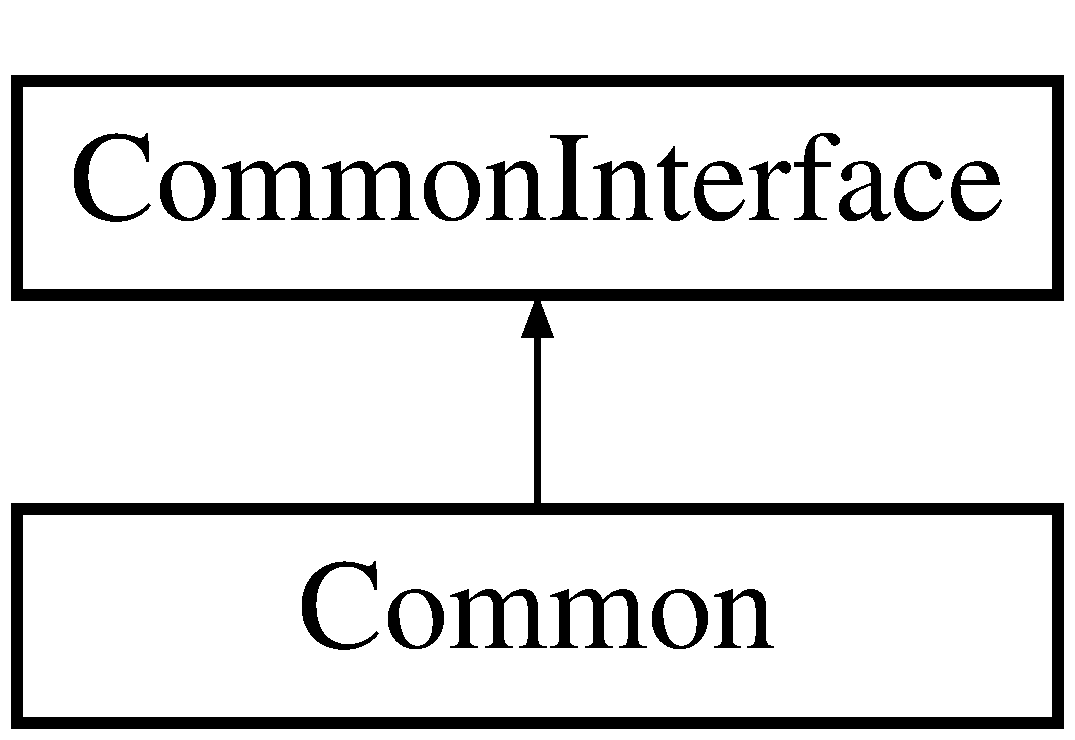
\includegraphics[height=2.000000cm]{class_common}
\end{center}
\end{figure}
\subsection*{Public Member Functions}
\begin{DoxyCompactItemize}
\item 
{\bf Common} (\$debug)
\item 
{\bf connect} (\$db)
\item 
{\bf execute\+Query} (\$sql, \$filename)
\end{DoxyCompactItemize}
\subsection*{Data Fields}
\begin{DoxyCompactItemize}
\item 
{\bf \$conn}
\item 
{\bf \$debug}
\item 
{\bf \$db} =\char`\"{}database.\+cse.\+tamu.\+edu\char`\"{}
\item 
{\bf \$dbname} =\char`\"{}jgwesterfield-\/Walker\+Data\char`\"{}
\item 
{\bf \$user} =\char`\"{}jgwesterfield\char`\"{}
\item 
{\bf \$pass} =\char`\"{}Whoop19!\char`\"{}
\end{DoxyCompactItemize}


\subsection{Detailed Description}
Created by Php\+Storm. User\+: Jonathan\+Westerfield Date\+: 2/8/18 Time\+: 4\+:20 PM 

Definition at line 9 of file Common\+Methods.\+php.



\subsection{Member Function Documentation}
\index{Common@{Common}!Common@{Common}}
\index{Common@{Common}!Common@{Common}}
\subsubsection[{Common(\$debug)}]{\setlength{\rightskip}{0pt plus 5cm}{\bf Common} (
\begin{DoxyParamCaption}
\item[{}]{\$debug}
\end{DoxyParamCaption}
)}\label{class_common_a4a9e6769ab6c946d0895e8d987df1c10}


Implements {\bf Common\+Interface} \doxyref{}{p.}{interface_common_interface_a4a9e6769ab6c946d0895e8d987df1c10}.



Definition at line 25 of file Common\+Methods.\+php.

\index{Common@{Common}!connect@{connect}}
\index{connect@{connect}!Common@{Common}}
\subsubsection[{connect(\$db)}]{\setlength{\rightskip}{0pt plus 5cm}connect (
\begin{DoxyParamCaption}
\item[{}]{\$db}
\end{DoxyParamCaption}
)}\label{class_common_a1b1bd9b3f45a5fbd2549355282cdc96f}


Implements {\bf Common\+Interface} \doxyref{}{p.}{interface_common_interface_a1b1bd9b3f45a5fbd2549355282cdc96f}.



Definition at line 34 of file Common\+Methods.\+php.

\index{Common@{Common}!execute\+Query@{execute\+Query}}
\index{execute\+Query@{execute\+Query}!Common@{Common}}
\subsubsection[{execute\+Query(\$sql, \$filename)}]{\setlength{\rightskip}{0pt plus 5cm}execute\+Query (
\begin{DoxyParamCaption}
\item[{}]{\$sql, }
\item[{}]{\$filename}
\end{DoxyParamCaption}
)}\label{class_common_a57a9dbd1203cf7b3ef3c5ce40d4047cc}


Implements {\bf Common\+Interface} \doxyref{}{p.}{interface_common_interface_a57a9dbd1203cf7b3ef3c5ce40d4047cc}.



Definition at line 49 of file Common\+Methods.\+php.



\subsection{Field Documentation}
\index{Common@{Common}!\$conn@{\$conn}}
\index{\$conn@{\$conn}!Common@{Common}}
\subsubsection[{\$conn}]{\setlength{\rightskip}{0pt plus 5cm}\$conn}\label{class_common_aa8a5a87b9c1a6a0819b88447cbe41877}


Definition at line 11 of file Common\+Methods.\+php.

\index{Common@{Common}!\$db@{\$db}}
\index{\$db@{\$db}!Common@{Common}}
\subsubsection[{\$db}]{\setlength{\rightskip}{0pt plus 5cm}\$db =\char`\"{}database.\+cse.\+tamu.\+edu\char`\"{}}\label{class_common_a1fa3127fc82f96b1436d871ef02be319}


Definition at line 20 of file Common\+Methods.\+php.

\index{Common@{Common}!\$dbname@{\$dbname}}
\index{\$dbname@{\$dbname}!Common@{Common}}
\subsubsection[{\$dbname}]{\setlength{\rightskip}{0pt plus 5cm}\$dbname =\char`\"{}jgwesterfield-\/Walker\+Data\char`\"{}}\label{class_common_ac5111a571fffa2499732833bb7f0d8c1}


Definition at line 21 of file Common\+Methods.\+php.

\index{Common@{Common}!\$debug@{\$debug}}
\index{\$debug@{\$debug}!Common@{Common}}
\subsubsection[{\$debug}]{\setlength{\rightskip}{0pt plus 5cm}\$debug}\label{class_common_a85ae3e64cd40e9564adceb010085e9dd}


Definition at line 12 of file Common\+Methods.\+php.

\index{Common@{Common}!\$pass@{\$pass}}
\index{\$pass@{\$pass}!Common@{Common}}
\subsubsection[{\$pass}]{\setlength{\rightskip}{0pt plus 5cm}\$pass =\char`\"{}Whoop19!\char`\"{}}\label{class_common_a12ec2780b52bd1c54d38c2f981c0349f}


Definition at line 23 of file Common\+Methods.\+php.

\index{Common@{Common}!\$user@{\$user}}
\index{\$user@{\$user}!Common@{Common}}
\subsubsection[{\$user}]{\setlength{\rightskip}{0pt plus 5cm}\$user =\char`\"{}jgwesterfield\char`\"{}}\label{class_common_a598ca4e71b15a1313ec95f0df1027ca5}


Definition at line 22 of file Common\+Methods.\+php.



The documentation for this class was generated from the following file\+:\begin{DoxyCompactItemize}
\item 
Users/\+Jonathan\+Westerfield/\+Documents/\+C\+S\+C\+E 315/\+Rec\+Walker\+Counter/{\bf Common\+Methods.\+php}\end{DoxyCompactItemize}

\section{Common\+Interface Interface Reference}
\label{interface_common_interface}\index{Common\+Interface@{Common\+Interface}}
Inheritance diagram for Common\+Interface\+:\begin{figure}[H]
\begin{center}
\leavevmode
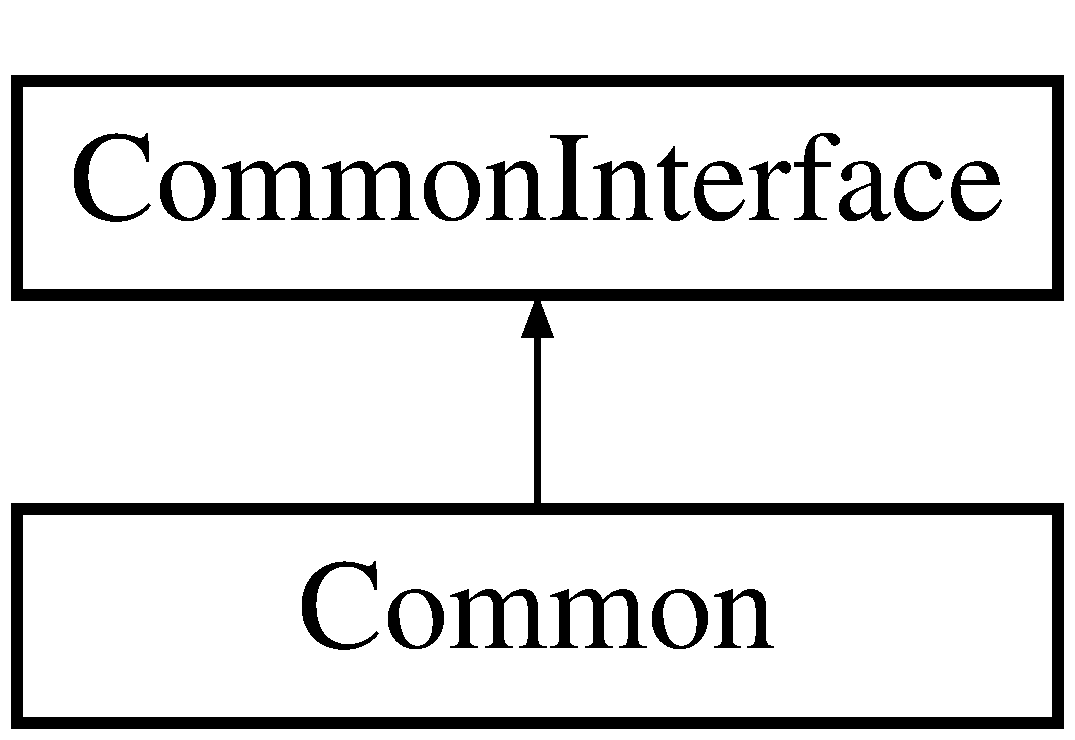
\includegraphics[height=2.000000cm]{interface_common_interface}
\end{center}
\end{figure}
\subsection*{Public Member Functions}
\begin{DoxyCompactItemize}
\item 
{\bfseries Common} (\$debug)\label{interface_common_interface_a4a9e6769ab6c946d0895e8d987df1c10}

\item 
{\bfseries connect} (\$db)\label{interface_common_interface_a1b1bd9b3f45a5fbd2549355282cdc96f}

\item 
{\bfseries execute\+Query} (\$sql, \$filename)\label{interface_common_interface_a57a9dbd1203cf7b3ef3c5ce40d4047cc}

\end{DoxyCompactItemize}


\subsection{Detailed Description}
Created by Php\+Storm. User\+: Jonathan\+Westerfield Date\+: 2/8/18 Time\+: 4\+:31 PM

This is an interface for \doxyref{Common}{p.}{class_common}. 

The documentation for this interface was generated from the following file\+:\begin{DoxyCompactItemize}
\item 
P\+H\+P\+:\+Mysql A\+P\+I/Common\+Interface.\+php\end{DoxyCompactItemize}

\section{D\+B\+A\+PI Class Reference}
\label{class_d_b_a_p_i}\index{D\+B\+A\+PI@{D\+B\+A\+PI}}
Inheritance diagram for D\+B\+A\+PI\+:\begin{figure}[H]
\begin{center}
\leavevmode
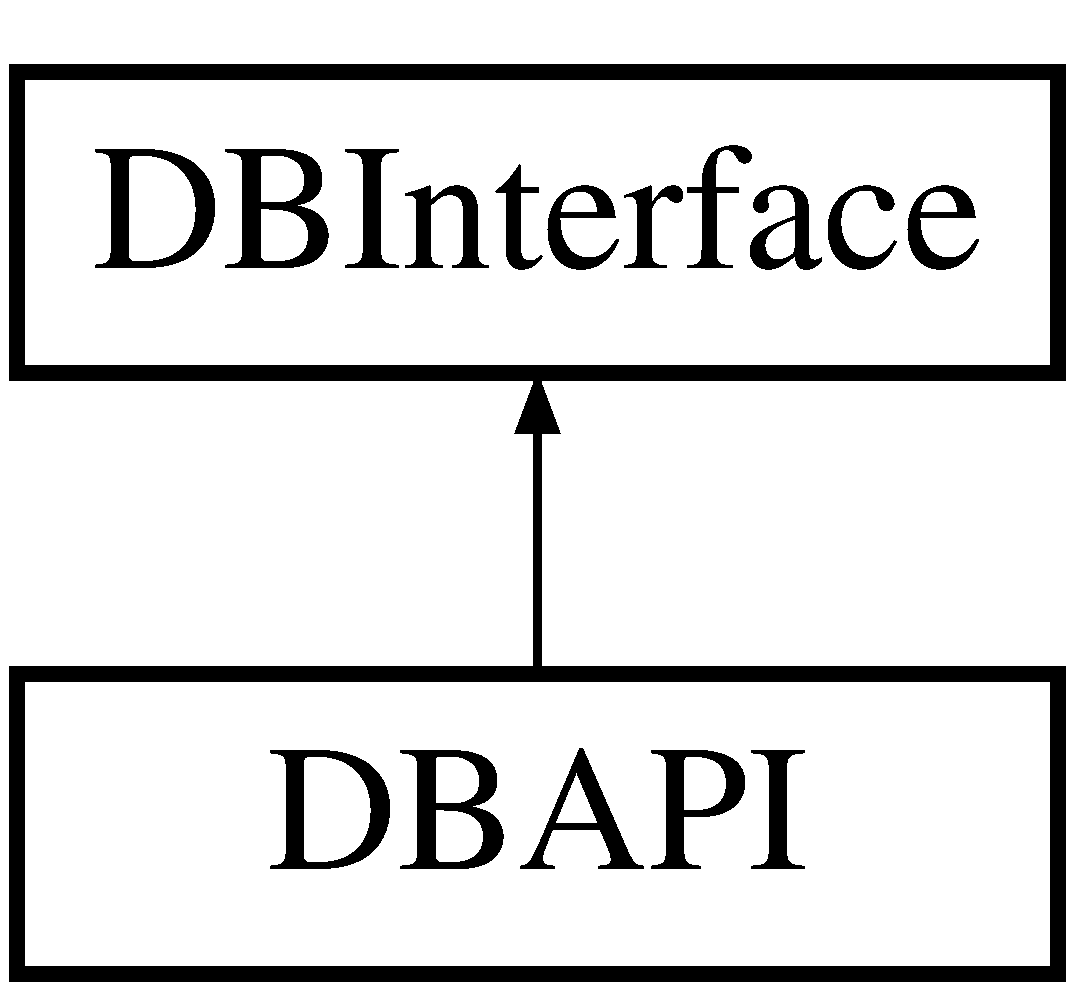
\includegraphics[height=2.000000cm]{class_d_b_a_p_i}
\end{center}
\end{figure}
\subsection*{Public Member Functions}
\begin{DoxyCompactItemize}
\item 
{\bf \+\_\+\+\_\+construct} (\$db)
\item 
{\bf \+\_\+\+\_\+destruct} ()
\item 
{\bf print\+Entire\+DB} ()
\item 
{\bf get\+Total\+Num\+Walkers} ()
\item 
{\bf get\+Num\+Walkers\+Today} ()
\item 
{\bf get\+Num\+Walkers\+This\+Week} ()
\item 
{\bf get\+Current\+Year\+Traffic} ()
\item 
{\bf get\+Traffic\+By\+Year} (\$year)
\item 
{\bf get\+Current\+Month\+Traffic} ()
\item 
{\bf get\+Traffic\+By\+Month} (\$year, \$month)
\item 
{\bf get\+Current\+Day\+Traffic} ()
\item 
{\bf get\+Traffic\+By\+Day} (\$year, \$month, \$day)
\item 
{\bf get\+Traffic\+Time\+Range} (\$year1, \$month1, \$day1, \$year2, \$month2, \$day2)
\end{DoxyCompactItemize}


\subsection{Detailed Description}
Created by Php\+Storm. User\+: Jonathan\+Westerfield Date\+: 2/8/18 Time\+: 4\+:35 PM

Includes the various functions that can be used in order to extract useful information from the database. Implements D\+B\+Interface.\+php 

\subsection{Constructor \& Destructor Documentation}
\index{D\+B\+A\+PI@{D\+B\+A\+PI}!\+\_\+\+\_\+construct@{\+\_\+\+\_\+construct}}
\index{\+\_\+\+\_\+construct@{\+\_\+\+\_\+construct}!D\+B\+A\+PI@{D\+B\+A\+PI}}
\subsubsection[{\+\_\+\+\_\+construct(\$db)}]{\setlength{\rightskip}{0pt plus 5cm}\+\_\+\+\_\+construct (
\begin{DoxyParamCaption}
\item[{}]{\$db}
\end{DoxyParamCaption}
)}\label{class_d_b_a_p_i_a800f8efee13692788b13ee57c5960092}
\doxyref{D\+B\+A\+PI}{p.}{class_d_b_a_p_i} constructor. 
\begin{DoxyParams}{Parameters}
{\em \$db} & Mostly sets up the dates in this object. Also sets the timezone to our timezone. \\
\hline
\end{DoxyParams}


Implements {\bf D\+B\+Interface} \doxyref{}{p.}{interface_d_b_interface_a800f8efee13692788b13ee57c5960092}.

\index{D\+B\+A\+PI@{D\+B\+A\+PI}!\+\_\+\+\_\+destruct@{\+\_\+\+\_\+destruct}}
\index{\+\_\+\+\_\+destruct@{\+\_\+\+\_\+destruct}!D\+B\+A\+PI@{D\+B\+A\+PI}}
\subsubsection[{\+\_\+\+\_\+destruct()}]{\setlength{\rightskip}{0pt plus 5cm}\+\_\+\+\_\+destruct (
\begin{DoxyParamCaption}
{}
\end{DoxyParamCaption}
)}\label{class_d_b_a_p_i_a421831a265621325e1fdd19aace0c758}
Class destructor 

Implements {\bf D\+B\+Interface} \doxyref{}{p.}{interface_d_b_interface}.



\subsection{Member Function Documentation}
\index{D\+B\+A\+PI@{D\+B\+A\+PI}!get\+Current\+Day\+Traffic@{get\+Current\+Day\+Traffic}}
\index{get\+Current\+Day\+Traffic@{get\+Current\+Day\+Traffic}!D\+B\+A\+PI@{D\+B\+A\+PI}}
\subsubsection[{get\+Current\+Day\+Traffic()}]{\setlength{\rightskip}{0pt plus 5cm}get\+Current\+Day\+Traffic (
\begin{DoxyParamCaption}
{}
\end{DoxyParamCaption}
)}\label{class_d_b_a_p_i_a50aa5202dd6a6314b4b0da6fd3026415}
\begin{DoxyReturn}{Returns}
array
\end{DoxyReturn}
Gets the number of people for every hour and returns a length 24 array output the times to see if I overshot how many times to iterate 

Implements {\bf D\+B\+Interface} \doxyref{}{p.}{interface_d_b_interface_a50aa5202dd6a6314b4b0da6fd3026415}.

\index{D\+B\+A\+PI@{D\+B\+A\+PI}!get\+Current\+Month\+Traffic@{get\+Current\+Month\+Traffic}}
\index{get\+Current\+Month\+Traffic@{get\+Current\+Month\+Traffic}!D\+B\+A\+PI@{D\+B\+A\+PI}}
\subsubsection[{get\+Current\+Month\+Traffic()}]{\setlength{\rightskip}{0pt plus 5cm}get\+Current\+Month\+Traffic (
\begin{DoxyParamCaption}
{}
\end{DoxyParamCaption}
)}\label{class_d_b_a_p_i_ae1b5c3c8112356b5c8ea9184286ec89a}
\begin{DoxyReturn}{Returns}
array
\end{DoxyReturn}
Gets the traffic numbers for each day during the current month. 

Implements {\bf D\+B\+Interface} \doxyref{}{p.}{interface_d_b_interface_ae1b5c3c8112356b5c8ea9184286ec89a}.

\index{D\+B\+A\+PI@{D\+B\+A\+PI}!get\+Current\+Year\+Traffic@{get\+Current\+Year\+Traffic}}
\index{get\+Current\+Year\+Traffic@{get\+Current\+Year\+Traffic}!D\+B\+A\+PI@{D\+B\+A\+PI}}
\subsubsection[{get\+Current\+Year\+Traffic()}]{\setlength{\rightskip}{0pt plus 5cm}get\+Current\+Year\+Traffic (
\begin{DoxyParamCaption}
{}
\end{DoxyParamCaption}
)}\label{class_d_b_a_p_i_ad487abf76c66536778a43009612b6843}
\begin{DoxyReturn}{Returns}
array
\end{DoxyReturn}
Returns an array of the traffic numbers for each month in a 12 element array 

Implements {\bf D\+B\+Interface} \doxyref{}{p.}{interface_d_b_interface_ad487abf76c66536778a43009612b6843}.

\index{D\+B\+A\+PI@{D\+B\+A\+PI}!get\+Num\+Walkers\+This\+Week@{get\+Num\+Walkers\+This\+Week}}
\index{get\+Num\+Walkers\+This\+Week@{get\+Num\+Walkers\+This\+Week}!D\+B\+A\+PI@{D\+B\+A\+PI}}
\subsubsection[{get\+Num\+Walkers\+This\+Week()}]{\setlength{\rightskip}{0pt plus 5cm}get\+Num\+Walkers\+This\+Week (
\begin{DoxyParamCaption}
{}
\end{DoxyParamCaption}
)}\label{class_d_b_a_p_i_ae7a2342889cfd984513ba17ddbd14bef}
\begin{DoxyReturn}{Returns}
int
\end{DoxyReturn}
Gets the number of walkers in the last week starting from today 

Implements {\bf D\+B\+Interface} \doxyref{}{p.}{interface_d_b_interface_ae7a2342889cfd984513ba17ddbd14bef}.

\index{D\+B\+A\+PI@{D\+B\+A\+PI}!get\+Num\+Walkers\+Today@{get\+Num\+Walkers\+Today}}
\index{get\+Num\+Walkers\+Today@{get\+Num\+Walkers\+Today}!D\+B\+A\+PI@{D\+B\+A\+PI}}
\subsubsection[{get\+Num\+Walkers\+Today()}]{\setlength{\rightskip}{0pt plus 5cm}get\+Num\+Walkers\+Today (
\begin{DoxyParamCaption}
{}
\end{DoxyParamCaption}
)}\label{class_d_b_a_p_i_adf40141a9763141c0eaeb9ce620181ad}
\begin{DoxyReturn}{Returns}
int
\end{DoxyReturn}
Gets the number of walkers from Today 

Implements {\bf D\+B\+Interface} \doxyref{}{p.}{interface_d_b_interface_adf40141a9763141c0eaeb9ce620181ad}.

\index{D\+B\+A\+PI@{D\+B\+A\+PI}!get\+Total\+Num\+Walkers@{get\+Total\+Num\+Walkers}}
\index{get\+Total\+Num\+Walkers@{get\+Total\+Num\+Walkers}!D\+B\+A\+PI@{D\+B\+A\+PI}}
\subsubsection[{get\+Total\+Num\+Walkers()}]{\setlength{\rightskip}{0pt plus 5cm}get\+Total\+Num\+Walkers (
\begin{DoxyParamCaption}
{}
\end{DoxyParamCaption}
)}\label{class_d_b_a_p_i_ab7a902c85d04b9973a30b73963cb3270}
\begin{DoxyReturn}{Returns}
int
\end{DoxyReturn}
Gets the total number of walkers in the table 

Implements {\bf D\+B\+Interface} \doxyref{}{p.}{interface_d_b_interface_ab7a902c85d04b9973a30b73963cb3270}.

\index{D\+B\+A\+PI@{D\+B\+A\+PI}!get\+Traffic\+By\+Day@{get\+Traffic\+By\+Day}}
\index{get\+Traffic\+By\+Day@{get\+Traffic\+By\+Day}!D\+B\+A\+PI@{D\+B\+A\+PI}}
\subsubsection[{get\+Traffic\+By\+Day(\$year, \$month, \$day)}]{\setlength{\rightskip}{0pt plus 5cm}get\+Traffic\+By\+Day (
\begin{DoxyParamCaption}
\item[{}]{\$year, }
\item[{}]{\$month, }
\item[{}]{\$day}
\end{DoxyParamCaption}
)}\label{class_d_b_a_p_i_a732a3a52aedfb5dd4b63f7292cb8ec3b}

\begin{DoxyParams}{Parameters}
{\em \$year} & \\
\hline
{\em \$month} & \\
\hline
{\em \$day} & \\
\hline
\end{DoxyParams}
\begin{DoxyReturn}{Returns}
array
\end{DoxyReturn}
Gets the traffic for each hour and returns it in a 24 element array.

Usage\+: $<$var = get\+Traffic\+By\+Day(2018, 2, 15);$>$ for Febraury 15, 2018 output the times to see if I overshot how many times to iterate 

Implements {\bf D\+B\+Interface} \doxyref{}{p.}{interface_d_b_interface_a732a3a52aedfb5dd4b63f7292cb8ec3b}.

\index{D\+B\+A\+PI@{D\+B\+A\+PI}!get\+Traffic\+By\+Month@{get\+Traffic\+By\+Month}}
\index{get\+Traffic\+By\+Month@{get\+Traffic\+By\+Month}!D\+B\+A\+PI@{D\+B\+A\+PI}}
\subsubsection[{get\+Traffic\+By\+Month(\$year, \$month)}]{\setlength{\rightskip}{0pt plus 5cm}get\+Traffic\+By\+Month (
\begin{DoxyParamCaption}
\item[{}]{\$year, }
\item[{}]{\$month}
\end{DoxyParamCaption}
)}\label{class_d_b_a_p_i_a0e954fca184f4b8ac04f51cb0c558def}

\begin{DoxyParams}{Parameters}
{\em \$year} & \\
\hline
{\em \$month} & \\
\hline
\end{DoxyParams}
\begin{DoxyReturn}{Returns}
array
\end{DoxyReturn}
Gets the traffic for each day during the specified month of the specified year

Usage\+: get\+Traffic\+By\+Month(2018, 2); // for February 2018 

Implements {\bf D\+B\+Interface} \doxyref{}{p.}{interface_d_b_interface_a0e954fca184f4b8ac04f51cb0c558def}.

\index{D\+B\+A\+PI@{D\+B\+A\+PI}!get\+Traffic\+By\+Year@{get\+Traffic\+By\+Year}}
\index{get\+Traffic\+By\+Year@{get\+Traffic\+By\+Year}!D\+B\+A\+PI@{D\+B\+A\+PI}}
\subsubsection[{get\+Traffic\+By\+Year(\$year)}]{\setlength{\rightskip}{0pt plus 5cm}get\+Traffic\+By\+Year (
\begin{DoxyParamCaption}
\item[{}]{\$year}
\end{DoxyParamCaption}
)}\label{class_d_b_a_p_i_a82c5e558141dca62c793baf0d1216bc0}

\begin{DoxyParams}{Parameters}
{\em \$year} & \\
\hline
\end{DoxyParams}
\begin{DoxyReturn}{Returns}
array
\end{DoxyReturn}
Gives the traffic for each month in an array for the specified year passed in 

Implements {\bf D\+B\+Interface} \doxyref{}{p.}{interface_d_b_interface_a82c5e558141dca62c793baf0d1216bc0}.

\index{D\+B\+A\+PI@{D\+B\+A\+PI}!get\+Traffic\+Time\+Range@{get\+Traffic\+Time\+Range}}
\index{get\+Traffic\+Time\+Range@{get\+Traffic\+Time\+Range}!D\+B\+A\+PI@{D\+B\+A\+PI}}
\subsubsection[{get\+Traffic\+Time\+Range(\$year1, \$month1, \$day1, \$year2, \$month2, \$day2)}]{\setlength{\rightskip}{0pt plus 5cm}get\+Traffic\+Time\+Range (
\begin{DoxyParamCaption}
\item[{}]{\$year1, }
\item[{}]{\$month1, }
\item[{}]{\$day1, }
\item[{}]{\$year2, }
\item[{}]{\$month2, }
\item[{}]{\$day2}
\end{DoxyParamCaption}
)}\label{class_d_b_a_p_i_a546615c71715e031c6218799e97937ab}

\begin{DoxyParams}{Parameters}
{\em \$year1} & \\
\hline
{\em \$month1} & \\
\hline
{\em \$day1} & \\
\hline
{\em \$year2} & \\
\hline
{\em \$month2} & \\
\hline
{\em \$day2} & \\
\hline
\end{DoxyParams}
\begin{DoxyReturn}{Returns}
int
\end{DoxyReturn}
Takes in a date range (start and end date) and counts the number of walkers in the given range 

Implements {\bf D\+B\+Interface} \doxyref{}{p.}{interface_d_b_interface_a546615c71715e031c6218799e97937ab}.

\index{D\+B\+A\+PI@{D\+B\+A\+PI}!print\+Entire\+DB@{print\+Entire\+DB}}
\index{print\+Entire\+DB@{print\+Entire\+DB}!D\+B\+A\+PI@{D\+B\+A\+PI}}
\subsubsection[{print\+Entire\+D\+B()}]{\setlength{\rightskip}{0pt plus 5cm}print\+Entire\+DB (
\begin{DoxyParamCaption}
{}
\end{DoxyParamCaption}
)}\label{class_d_b_a_p_i_a7e02b55449fecf4bed4ca717f38dafd5}
Prints out a table of the entire database 

Implements {\bf D\+B\+Interface} \doxyref{}{p.}{interface_d_b_interface}.



The documentation for this class was generated from the following file\+:\begin{DoxyCompactItemize}
\item 
P\+H\+P\+:\+Mysql A\+P\+I/D\+B\+A\+P\+I.\+php\end{DoxyCompactItemize}

\section{D\+B\+Interface Interface Reference}
\label{interface_d_b_interface}\index{D\+B\+Interface@{D\+B\+Interface}}
Inheritance diagram for D\+B\+Interface\+:\begin{figure}[H]
\begin{center}
\leavevmode
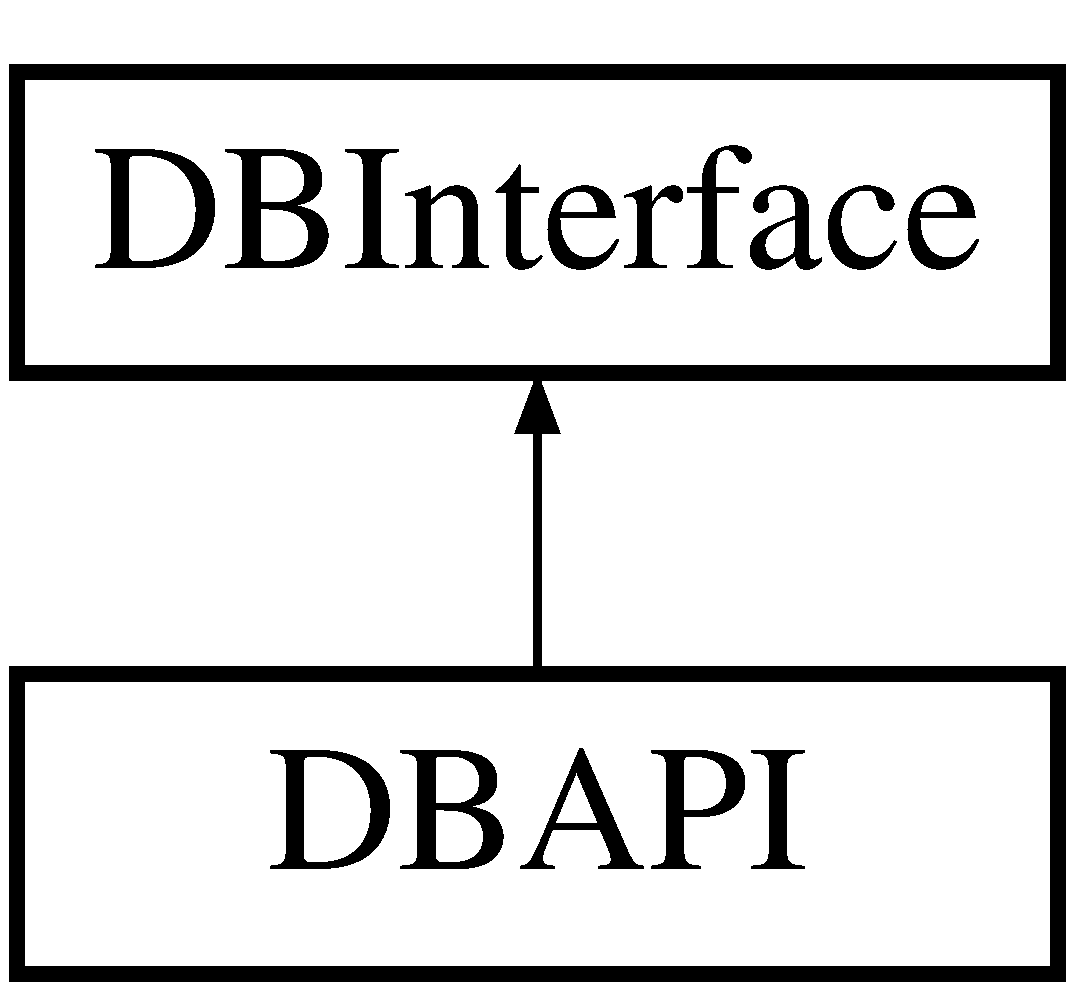
\includegraphics[height=2.000000cm]{interface_d_b_interface}
\end{center}
\end{figure}
\subsection*{Public Member Functions}
\begin{DoxyCompactItemize}
\item 
{\bf \+\_\+\+\_\+construct} (\$db)
\item 
{\bf \+\_\+\+\_\+destruct} ()
\item 
{\bf print\+Entire\+DB} ()
\item 
{\bf get\+Total\+Num\+Walkers} ()
\item 
{\bf get\+Num\+Walkers\+Today} ()
\item 
{\bf get\+Num\+Walkers\+This\+Week} ()
\item 
{\bf get\+Current\+Year\+Traffic} ()
\item 
{\bf get\+Traffic\+By\+Year} (\$year)
\item 
{\bf get\+Current\+Month\+Traffic} ()
\item 
{\bf get\+Traffic\+By\+Month} (\$year, \$month)
\item 
{\bf get\+Current\+Day\+Traffic} ()
\item 
{\bf get\+Traffic\+By\+Day} (\$year, \$month, \$day)
\item 
{\bf get\+Traffic\+Time\+Range} (\$year1, \$month1, \$day1, \$year2, \$month2, \$day2)
\end{DoxyCompactItemize}


\subsection{Detailed Description}
Created by Php\+Storm. User\+: Jonathan\+Westerfield Date\+: 2/8/18 Time\+: 4\+:36 PM 

Definition at line 11 of file D\+B\+Interface.\+php.



\subsection{Constructor \& Destructor Documentation}
\index{D\+B\+Interface@{D\+B\+Interface}!\+\_\+\+\_\+construct@{\+\_\+\+\_\+construct}}
\index{\+\_\+\+\_\+construct@{\+\_\+\+\_\+construct}!D\+B\+Interface@{D\+B\+Interface}}
\subsubsection[{\+\_\+\+\_\+construct(\$db)}]{\setlength{\rightskip}{0pt plus 5cm}\+\_\+\+\_\+construct (
\begin{DoxyParamCaption}
\item[{}]{\$db}
\end{DoxyParamCaption}
)}\label{interface_d_b_interface_a800f8efee13692788b13ee57c5960092}
\doxyref{D\+B\+A\+PI}{p.}{class_d_b_a_p_i} constructor. 
\begin{DoxyParams}{Parameters}
{\em \$db} & Mostly sets up the dates in this object. Also sets the timezone to our timezone. \\
\hline
\end{DoxyParams}


Implemented in {\bf D\+B\+A\+PI} \doxyref{}{p.}{class_d_b_a_p_i_a800f8efee13692788b13ee57c5960092}.

\index{D\+B\+Interface@{D\+B\+Interface}!\+\_\+\+\_\+destruct@{\+\_\+\+\_\+destruct}}
\index{\+\_\+\+\_\+destruct@{\+\_\+\+\_\+destruct}!D\+B\+Interface@{D\+B\+Interface}}
\subsubsection[{\+\_\+\+\_\+destruct()}]{\setlength{\rightskip}{0pt plus 5cm}\+\_\+\+\_\+destruct (
\begin{DoxyParamCaption}
{}
\end{DoxyParamCaption}
)}\label{interface_d_b_interface_a421831a265621325e1fdd19aace0c758}


Implemented in {\bf D\+B\+A\+PI} \doxyref{}{p.}{class_d_b_a_p_i_a421831a265621325e1fdd19aace0c758}.



\subsection{Member Function Documentation}
\index{D\+B\+Interface@{D\+B\+Interface}!get\+Current\+Day\+Traffic@{get\+Current\+Day\+Traffic}}
\index{get\+Current\+Day\+Traffic@{get\+Current\+Day\+Traffic}!D\+B\+Interface@{D\+B\+Interface}}
\subsubsection[{get\+Current\+Day\+Traffic()}]{\setlength{\rightskip}{0pt plus 5cm}get\+Current\+Day\+Traffic (
\begin{DoxyParamCaption}
{}
\end{DoxyParamCaption}
)}\label{interface_d_b_interface_a50aa5202dd6a6314b4b0da6fd3026415}
\begin{DoxyReturn}{Returns}
array
\end{DoxyReturn}
Returns a length 24 array containing total number of walkers for each hour for the current day 

Implemented in {\bf D\+B\+A\+PI} \doxyref{}{p.}{class_d_b_a_p_i_a50aa5202dd6a6314b4b0da6fd3026415}.

\index{D\+B\+Interface@{D\+B\+Interface}!get\+Current\+Month\+Traffic@{get\+Current\+Month\+Traffic}}
\index{get\+Current\+Month\+Traffic@{get\+Current\+Month\+Traffic}!D\+B\+Interface@{D\+B\+Interface}}
\subsubsection[{get\+Current\+Month\+Traffic()}]{\setlength{\rightskip}{0pt plus 5cm}get\+Current\+Month\+Traffic (
\begin{DoxyParamCaption}
{}
\end{DoxyParamCaption}
)}\label{interface_d_b_interface_ae1b5c3c8112356b5c8ea9184286ec89a}
\begin{DoxyReturn}{Returns}
array
\end{DoxyReturn}
Returns an array containing total number of walkers for each day for the current month 

Implemented in {\bf D\+B\+A\+PI} \doxyref{}{p.}{class_d_b_a_p_i_ae1b5c3c8112356b5c8ea9184286ec89a}.

\index{D\+B\+Interface@{D\+B\+Interface}!get\+Current\+Year\+Traffic@{get\+Current\+Year\+Traffic}}
\index{get\+Current\+Year\+Traffic@{get\+Current\+Year\+Traffic}!D\+B\+Interface@{D\+B\+Interface}}
\subsubsection[{get\+Current\+Year\+Traffic()}]{\setlength{\rightskip}{0pt plus 5cm}get\+Current\+Year\+Traffic (
\begin{DoxyParamCaption}
{}
\end{DoxyParamCaption}
)}\label{interface_d_b_interface_ad487abf76c66536778a43009612b6843}
\begin{DoxyReturn}{Returns}
array
\end{DoxyReturn}
Returns an array containing total number of walkers for each month for the current year 12 Element Array 

Implemented in {\bf D\+B\+A\+PI} \doxyref{}{p.}{class_d_b_a_p_i_ad487abf76c66536778a43009612b6843}.

\index{D\+B\+Interface@{D\+B\+Interface}!get\+Num\+Walkers\+This\+Week@{get\+Num\+Walkers\+This\+Week}}
\index{get\+Num\+Walkers\+This\+Week@{get\+Num\+Walkers\+This\+Week}!D\+B\+Interface@{D\+B\+Interface}}
\subsubsection[{get\+Num\+Walkers\+This\+Week()}]{\setlength{\rightskip}{0pt plus 5cm}get\+Num\+Walkers\+This\+Week (
\begin{DoxyParamCaption}
{}
\end{DoxyParamCaption}
)}\label{interface_d_b_interface_ae7a2342889cfd984513ba17ddbd14bef}
\begin{DoxyReturn}{Returns}
int
\end{DoxyReturn}
Returns the number of walkers from the start to the end of the week 

Implemented in {\bf D\+B\+A\+PI} \doxyref{}{p.}{class_d_b_a_p_i_ae7a2342889cfd984513ba17ddbd14bef}.

\index{D\+B\+Interface@{D\+B\+Interface}!get\+Num\+Walkers\+Today@{get\+Num\+Walkers\+Today}}
\index{get\+Num\+Walkers\+Today@{get\+Num\+Walkers\+Today}!D\+B\+Interface@{D\+B\+Interface}}
\subsubsection[{get\+Num\+Walkers\+Today()}]{\setlength{\rightskip}{0pt plus 5cm}get\+Num\+Walkers\+Today (
\begin{DoxyParamCaption}
{}
\end{DoxyParamCaption}
)}\label{interface_d_b_interface_adf40141a9763141c0eaeb9ce620181ad}
\begin{DoxyReturn}{Returns}
int
\end{DoxyReturn}
Returns the number of walkers that walked through from the start to the end of the day 

Implemented in {\bf D\+B\+A\+PI} \doxyref{}{p.}{class_d_b_a_p_i_adf40141a9763141c0eaeb9ce620181ad}.

\index{D\+B\+Interface@{D\+B\+Interface}!get\+Total\+Num\+Walkers@{get\+Total\+Num\+Walkers}}
\index{get\+Total\+Num\+Walkers@{get\+Total\+Num\+Walkers}!D\+B\+Interface@{D\+B\+Interface}}
\subsubsection[{get\+Total\+Num\+Walkers()}]{\setlength{\rightskip}{0pt plus 5cm}get\+Total\+Num\+Walkers (
\begin{DoxyParamCaption}
{}
\end{DoxyParamCaption}
)}\label{interface_d_b_interface_ab7a902c85d04b9973a30b73963cb3270}
\begin{DoxyReturn}{Returns}
int
\end{DoxyReturn}
Returns the total number of walkers in the table 

Implemented in {\bf D\+B\+A\+PI} \doxyref{}{p.}{class_d_b_a_p_i_ab7a902c85d04b9973a30b73963cb3270}.

\index{D\+B\+Interface@{D\+B\+Interface}!get\+Traffic\+By\+Day@{get\+Traffic\+By\+Day}}
\index{get\+Traffic\+By\+Day@{get\+Traffic\+By\+Day}!D\+B\+Interface@{D\+B\+Interface}}
\subsubsection[{get\+Traffic\+By\+Day(\$year, \$month, \$day)}]{\setlength{\rightskip}{0pt plus 5cm}get\+Traffic\+By\+Day (
\begin{DoxyParamCaption}
\item[{}]{\$year, }
\item[{}]{\$month, }
\item[{}]{\$day}
\end{DoxyParamCaption}
)}\label{interface_d_b_interface_a732a3a52aedfb5dd4b63f7292cb8ec3b}

\begin{DoxyParams}{Parameters}
{\em \$year} & \\
\hline
{\em \$month} & \\
\hline
{\em \$day} & \\
\hline
\end{DoxyParams}
\begin{DoxyReturn}{Returns}
array
\end{DoxyReturn}
Returns an array (24) containing total number of walkers for each hour

Usage\+: $<$var = get\+Traffic\+By\+Day(2018, 2, 15);$>$ for Febraury 15, 2018 

Implemented in {\bf D\+B\+A\+PI} \doxyref{}{p.}{class_d_b_a_p_i_a732a3a52aedfb5dd4b63f7292cb8ec3b}.

\index{D\+B\+Interface@{D\+B\+Interface}!get\+Traffic\+By\+Month@{get\+Traffic\+By\+Month}}
\index{get\+Traffic\+By\+Month@{get\+Traffic\+By\+Month}!D\+B\+Interface@{D\+B\+Interface}}
\subsubsection[{get\+Traffic\+By\+Month(\$year, \$month)}]{\setlength{\rightskip}{0pt plus 5cm}get\+Traffic\+By\+Month (
\begin{DoxyParamCaption}
\item[{}]{\$year, }
\item[{}]{\$month}
\end{DoxyParamCaption}
)}\label{interface_d_b_interface_a0e954fca184f4b8ac04f51cb0c558def}

\begin{DoxyParams}{Parameters}
{\em \$year} & \\
\hline
{\em \$month} & \\
\hline
\end{DoxyParams}
\begin{DoxyReturn}{Returns}
array
\end{DoxyReturn}
Gets the traffic for each day during the specified month of the specified year

Usage\+: get\+Traffic\+By\+Month(2018, 2); // for February 2018 

Implemented in {\bf D\+B\+A\+PI} \doxyref{}{p.}{class_d_b_a_p_i_a0e954fca184f4b8ac04f51cb0c558def}.

\index{D\+B\+Interface@{D\+B\+Interface}!get\+Traffic\+By\+Year@{get\+Traffic\+By\+Year}}
\index{get\+Traffic\+By\+Year@{get\+Traffic\+By\+Year}!D\+B\+Interface@{D\+B\+Interface}}
\subsubsection[{get\+Traffic\+By\+Year(\$year)}]{\setlength{\rightskip}{0pt plus 5cm}get\+Traffic\+By\+Year (
\begin{DoxyParamCaption}
\item[{}]{\$year}
\end{DoxyParamCaption}
)}\label{interface_d_b_interface_a82c5e558141dca62c793baf0d1216bc0}

\begin{DoxyParams}{Parameters}
{\em \$year} & \\
\hline
\end{DoxyParams}
\begin{DoxyReturn}{Returns}
array
\end{DoxyReturn}
Gives the traffic for each month in an array for the specified year passed in 

Implemented in {\bf D\+B\+A\+PI} \doxyref{}{p.}{class_d_b_a_p_i_a82c5e558141dca62c793baf0d1216bc0}.

\index{D\+B\+Interface@{D\+B\+Interface}!get\+Traffic\+Time\+Range@{get\+Traffic\+Time\+Range}}
\index{get\+Traffic\+Time\+Range@{get\+Traffic\+Time\+Range}!D\+B\+Interface@{D\+B\+Interface}}
\subsubsection[{get\+Traffic\+Time\+Range(\$year1, \$month1, \$day1, \$year2, \$month2, \$day2)}]{\setlength{\rightskip}{0pt plus 5cm}get\+Traffic\+Time\+Range (
\begin{DoxyParamCaption}
\item[{}]{\$year1, }
\item[{}]{\$month1, }
\item[{}]{\$day1, }
\item[{}]{\$year2, }
\item[{}]{\$month2, }
\item[{}]{\$day2}
\end{DoxyParamCaption}
)}\label{interface_d_b_interface_a546615c71715e031c6218799e97937ab}

\begin{DoxyParams}{Parameters}
{\em \$year1} & \\
\hline
{\em \$month1} & \\
\hline
{\em \$day1} & \\
\hline
{\em \$year2} & \\
\hline
{\em \$month2} & \\
\hline
{\em \$day2} & \\
\hline
\end{DoxyParams}
\begin{DoxyReturn}{Returns}
int
\end{DoxyReturn}
Takes in a date range (start and end date) and counts the number of walkers in the given range 

Implemented in {\bf D\+B\+A\+PI} \doxyref{}{p.}{class_d_b_a_p_i_a546615c71715e031c6218799e97937ab}.

\index{D\+B\+Interface@{D\+B\+Interface}!print\+Entire\+DB@{print\+Entire\+DB}}
\index{print\+Entire\+DB@{print\+Entire\+DB}!D\+B\+Interface@{D\+B\+Interface}}
\subsubsection[{print\+Entire\+D\+B()}]{\setlength{\rightskip}{0pt plus 5cm}print\+Entire\+DB (
\begin{DoxyParamCaption}
{}
\end{DoxyParamCaption}
)}\label{interface_d_b_interface_a7e02b55449fecf4bed4ca717f38dafd5}


Implemented in {\bf D\+B\+A\+PI} \doxyref{}{p.}{class_d_b_a_p_i_a7e02b55449fecf4bed4ca717f38dafd5}.



The documentation for this interface was generated from the following file\+:\begin{DoxyCompactItemize}
\item 
{\bf D\+B\+Interface.\+php}\end{DoxyCompactItemize}

\section{P\+D\+B\+A\+PI Class Reference}
\label{class_p_d_b_a_p_i_1_1_p_d_b_a_p_i}\index{P\+D\+B\+A\+PI@{P\+D\+B\+A\+PI}}
\subsection*{Public Member Functions}
\begin{DoxyCompactItemize}
\item 
def {\bf \+\_\+\+\_\+init\+\_\+\+\_\+} (self)
\item 
def {\bf \+\_\+\+\_\+del\+\_\+\+\_\+} (self)
\item 
def {\bf insert} (self, in\+Or\+Out)
\end{DoxyCompactItemize}


\subsection{Detailed Description}


Definition at line 4 of file P\+D\+B\+A\+P\+I.\+py.



\subsection{Constructor \& Destructor Documentation}
\index{P\+D\+B\+A\+P\+I\+::\+P\+D\+B\+A\+PI@{P\+D\+B\+A\+P\+I\+::\+P\+D\+B\+A\+PI}!\+\_\+\+\_\+init\+\_\+\+\_\+@{\+\_\+\+\_\+init\+\_\+\+\_\+}}
\index{\+\_\+\+\_\+init\+\_\+\+\_\+@{\+\_\+\+\_\+init\+\_\+\+\_\+}!P\+D\+B\+A\+P\+I\+::\+P\+D\+B\+A\+PI@{P\+D\+B\+A\+P\+I\+::\+P\+D\+B\+A\+PI}}
\subsubsection[{\+\_\+\+\_\+init\+\_\+\+\_\+(self)}]{\setlength{\rightskip}{0pt plus 5cm}def \+\_\+\+\_\+init\+\_\+\+\_\+ (
\begin{DoxyParamCaption}
\item[{}]{self}
\end{DoxyParamCaption}
)}\label{class_p_d_b_a_p_i_1_1_p_d_b_a_p_i_ae64f0875afe3067b97ba370b354b9213}


Definition at line 13 of file P\+D\+B\+A\+P\+I.\+py.

\index{P\+D\+B\+A\+P\+I\+::\+P\+D\+B\+A\+PI@{P\+D\+B\+A\+P\+I\+::\+P\+D\+B\+A\+PI}!\+\_\+\+\_\+del\+\_\+\+\_\+@{\+\_\+\+\_\+del\+\_\+\+\_\+}}
\index{\+\_\+\+\_\+del\+\_\+\+\_\+@{\+\_\+\+\_\+del\+\_\+\+\_\+}!P\+D\+B\+A\+P\+I\+::\+P\+D\+B\+A\+PI@{P\+D\+B\+A\+P\+I\+::\+P\+D\+B\+A\+PI}}
\subsubsection[{\+\_\+\+\_\+del\+\_\+\+\_\+(self)}]{\setlength{\rightskip}{0pt plus 5cm}def \+\_\+\+\_\+del\+\_\+\+\_\+ (
\begin{DoxyParamCaption}
\item[{}]{self}
\end{DoxyParamCaption}
)}\label{class_p_d_b_a_p_i_1_1_p_d_b_a_p_i_a41a65d7030dd1006b177d0bc24e1a12b}


Definition at line 28 of file P\+D\+B\+A\+P\+I.\+py.



\subsection{Member Function Documentation}
\index{P\+D\+B\+A\+P\+I\+::\+P\+D\+B\+A\+PI@{P\+D\+B\+A\+P\+I\+::\+P\+D\+B\+A\+PI}!insert@{insert}}
\index{insert@{insert}!P\+D\+B\+A\+P\+I\+::\+P\+D\+B\+A\+PI@{P\+D\+B\+A\+P\+I\+::\+P\+D\+B\+A\+PI}}
\subsubsection[{insert(self, in\+Or\+Out)}]{\setlength{\rightskip}{0pt plus 5cm}def insert (
\begin{DoxyParamCaption}
\item[{}]{self, }
\item[{}]{in\+Or\+Out}
\end{DoxyParamCaption}
)}\label{class_p_d_b_a_p_i_1_1_p_d_b_a_p_i_a92919dd1ba46f1db668faf16328afb40}


Definition at line 33 of file P\+D\+B\+A\+P\+I.\+py.



The documentation for this class was generated from the following file\+:\begin{DoxyCompactItemize}
\item 
Users/\+Jonathan\+Westerfield/\+Documents/\+C\+S\+C\+E 315/\+Rec\+Walker\+Counter/\+Python/{\bf P\+D\+B\+A\+P\+I.\+py}\end{DoxyCompactItemize}

\chapter{File Documentation}
\section{Users/\+Jonathan\+Westerfield/\+Documents/\+C\+S\+CE 315/\+Rec\+Walker\+Counter/\+Chart.min.\+js File Reference}
\label{_chart_8min_8js}\index{Users/\+Jonathan\+Westerfield/\+Documents/\+C\+S\+C\+E 315/\+Rec\+Walker\+Counter/\+Chart.\+min.\+js@{Users/\+Jonathan\+Westerfield/\+Documents/\+C\+S\+C\+E 315/\+Rec\+Walker\+Counter/\+Chart.\+min.\+js}}
\subsection*{Functions}
\begin{DoxyCompactItemize}
\item 
{\bf !function} ({\bf t})
\end{DoxyCompactItemize}


\subsection{Function Documentation}
\index{Chart.\+min.\+js@{Chart.\+min.\+js}!"!function@{"!function}}
\index{"!function@{"!function}!Chart.\+min.\+js@{Chart.\+min.\+js}}
\subsubsection[{"!function(t)}]{\setlength{\rightskip}{0pt plus 5cm}!function (
\begin{DoxyParamCaption}
\item[{}]{t}
\end{DoxyParamCaption}
)}\label{_chart_8min_8js_a6e2c9a4472a75ae2ec32ee54ff87c001}
Chart.\+js {\tt http\+://chartjs.\+org/} Version\+: 2.\+4.\+0

Copyright 2016 Nick Downie Released under the M\+IT license {\tt https\+://github.\+com/chartjs/\+Chart.\+js/blob/master/\+L\+I\+C\+E\+N\+S\+E.\+md} 

Definition at line 10 of file Chart.\+min.\+js.


\hypertarget{_common_interface_8php}{}\section{P\+H\+P-\/\+My\+S\+QL Source/\+Common\+Interface.php File Reference}
\label{_common_interface_8php}\index{P\+H\+P-\/\+My\+S\+Q\+L Source/\+Common\+Interface.\+php@{P\+H\+P-\/\+My\+S\+Q\+L Source/\+Common\+Interface.\+php}}
\subsection*{Data Structures}
\begin{DoxyCompactItemize}
\item 
interface \hyperlink{interface_common_interface}{Common\+Interface}
\end{DoxyCompactItemize}

\section{Common\+Methods.\+php File Reference}
\label{_common_methods_8php}\index{Common\+Methods.\+php@{Common\+Methods.\+php}}
\subsection*{Data Structures}
\begin{DoxyCompactItemize}
\item 
class {\bf Common}
\end{DoxyCompactItemize}

\hypertarget{_d_b_a_p_i_8php}{}\section{P\+H\+P-\/\+My\+S\+QL Source/\+D\+B\+A\+PI.php File Reference}
\label{_d_b_a_p_i_8php}\index{P\+H\+P-\/\+My\+S\+Q\+L Source/\+D\+B\+A\+P\+I.\+php@{P\+H\+P-\/\+My\+S\+Q\+L Source/\+D\+B\+A\+P\+I.\+php}}
\subsection*{Data Structures}
\begin{DoxyCompactItemize}
\item 
class \hyperlink{class_d_b_a_p_i}{D\+B\+A\+PI}
\end{DoxyCompactItemize}

\hypertarget{_d_b_interface_8php}{}\section{P\+H\+P-\/\+My\+S\+QL Source/\+D\+B\+Interface.php File Reference}
\label{_d_b_interface_8php}\index{P\+H\+P-\/\+My\+S\+Q\+L Source/\+D\+B\+Interface.\+php@{P\+H\+P-\/\+My\+S\+Q\+L Source/\+D\+B\+Interface.\+php}}
\subsection*{Data Structures}
\begin{DoxyCompactItemize}
\item 
interface \hyperlink{interface_d_b_interface}{D\+B\+Interface}
\end{DoxyCompactItemize}

\section{graph.\+php File Reference}
\label{graph_8php}\index{graph.\+php@{graph.\+php}}
\subsection*{Functions}
\begin{DoxyCompactItemize}
\item 
{\bf print\+\_\+array} (\$values)
\item 
{\bf display\+\_\+graph} (\$labels, \$values, \$date\+\_\+format)
\end{DoxyCompactItemize}
\subsection*{Variables}
\begin{DoxyCompactItemize}
\item 
{\bf \$this\+Common} = new {\bf Common}(true)
\item 
{\bf \$db} = new {\bf D\+B\+A\+PI}(\$this\+Common)
\item 
if(!isset(\$\+\_\+\+G\+ET[\textquotesingle{}mode\textquotesingle{}])) elseif(strtolower(\$\+\_\+\+G\+ET[\textquotesingle{}mode\textquotesingle{}])== \textquotesingle{}day\textquotesingle{}$\vert$$\vert$strtolower(\$\+\_\+\+G\+ET[\textquotesingle{}mode\textquotesingle{}])== \textquotesingle{}month\textquotesingle{}$\vert$$\vert$strtolower(\$\+\_\+\+G\+ET[\textquotesingle{}mode\textquotesingle{}])== \textquotesingle{}year\textquotesingle{}) {\bf else}
\end{DoxyCompactItemize}


\subsection{Function Documentation}
\index{graph.\+php@{graph.\+php}!display\+\_\+graph@{display\+\_\+graph}}
\index{display\+\_\+graph@{display\+\_\+graph}!graph.\+php@{graph.\+php}}
\subsubsection[{display\+\_\+graph(\$labels, \$values, \$date\+\_\+format)}]{\setlength{\rightskip}{0pt plus 5cm}display\+\_\+graph (
\begin{DoxyParamCaption}
\item[{}]{\$labels, }
\item[{}]{\$values, }
\item[{}]{\$date\+\_\+format}
\end{DoxyParamCaption}
)}\label{graph_8php_af55d8d11c9641c2dd1b0b29a790b0fe8}


Definition at line 24 of file graph.\+php.

\index{graph.\+php@{graph.\+php}!print\+\_\+array@{print\+\_\+array}}
\index{print\+\_\+array@{print\+\_\+array}!graph.\+php@{graph.\+php}}
\subsubsection[{print\+\_\+array(\$values)}]{\setlength{\rightskip}{0pt plus 5cm}print\+\_\+array (
\begin{DoxyParamCaption}
\item[{}]{\$values}
\end{DoxyParamCaption}
)}\label{graph_8php_a7af48d7091d5a774294eae9ab84a5057}


Definition at line 9 of file graph.\+php.



\subsection{Variable Documentation}
\index{graph.\+php@{graph.\+php}!\$db@{\$db}}
\index{\$db@{\$db}!graph.\+php@{graph.\+php}}
\subsubsection[{\$db}]{\setlength{\rightskip}{0pt plus 5cm}\$db = new {\bf D\+B\+A\+PI}(\$this\+Common)}\label{graph_8php_a1fa3127fc82f96b1436d871ef02be319}


Definition at line 7 of file graph.\+php.

\index{graph.\+php@{graph.\+php}!\$this\+Common@{\$this\+Common}}
\index{\$this\+Common@{\$this\+Common}!graph.\+php@{graph.\+php}}
\subsubsection[{\$this\+Common}]{\setlength{\rightskip}{0pt plus 5cm}\$this\+Common = new {\bf Common}(true)}\label{graph_8php_a2dc37683cec5a169d791007363950944}


Definition at line 6 of file graph.\+php.

\index{graph.\+php@{graph.\+php}!else@{else}}
\index{else@{else}!graph.\+php@{graph.\+php}}
\subsubsection[{else}]{\setlength{\rightskip}{0pt plus 5cm}if (!isset(\$\+\_\+\+G\+ET[\textquotesingle{}mode\textquotesingle{}])) elseif (strtolower(\$\+\_\+\+G\+ET[\textquotesingle{}mode\textquotesingle{}])== \textquotesingle{}day\textquotesingle{}$\vert$$\vert$strtolower(\$\+\_\+\+G\+ET[\textquotesingle{}mode\textquotesingle{}])== \textquotesingle{}month\textquotesingle{}$\vert$$\vert$strtolower(\$\+\_\+\+G\+ET[\textquotesingle{}mode\textquotesingle{}])== \textquotesingle{}year\textquotesingle{}) else}\label{graph_8php_aa98e5745136db21835880938c0eba666}
{\bfseries Initial value\+:}
\begin{DoxyCode}
\{

    echo \textcolor{stringliteral}{'<script>console.log("Could not load form with mode \(\backslash\)\(\backslash\)"'} . $\_GET[\textcolor{stringliteral}{'mode'}] . \textcolor{stringliteral}{'\(\backslash\)\(\backslash\)".");</script>'}
\end{DoxyCode}


Definition at line 106 of file graph.\+php.


\section{index.\+php File Reference}
\label{index_8php}\index{index.\+php@{index.\+php}}
\subsection*{Variables}
\begin{DoxyCompactItemize}
\item 
{\bf \$this\+Common} = new {\bf Common}(true)
\item 
{\bf \$db} = new {\bf D\+B\+A\+PI}(\$this\+Common)
\end{DoxyCompactItemize}


\subsection{Variable Documentation}
\index{index.\+php@{index.\+php}!\$db@{\$db}}
\index{\$db@{\$db}!index.\+php@{index.\+php}}
\subsubsection[{\$db}]{\setlength{\rightskip}{0pt plus 5cm}\$db = new {\bf D\+B\+A\+PI}(\$this\+Common)}\label{index_8php_a1fa3127fc82f96b1436d871ef02be319}


Definition at line 6 of file index.\+php.

\index{index.\+php@{index.\+php}!\$this\+Common@{\$this\+Common}}
\index{\$this\+Common@{\$this\+Common}!index.\+php@{index.\+php}}
\subsubsection[{\$this\+Common}]{\setlength{\rightskip}{0pt plus 5cm}\$this\+Common = new {\bf Common}(true)}\label{index_8php_a2dc37683cec5a169d791007363950944}


Definition at line 5 of file index.\+php.


\section{Users/\+Jonathan\+Westerfield/\+Documents/\+C\+S\+CE 315/\+Rec\+Walker\+Counter/jquery-\/3.3.1.min.\+js File Reference}
\label{jquery-3_83_81_8min_8js}\index{Users/\+Jonathan\+Westerfield/\+Documents/\+C\+S\+C\+E 315/\+Rec\+Walker\+Counter/jquery-\/3.\+3.\+1.\+min.\+js@{Users/\+Jonathan\+Westerfield/\+Documents/\+C\+S\+C\+E 315/\+Rec\+Walker\+Counter/jquery-\/3.\+3.\+1.\+min.\+js}}
\subsection*{Functions}
\begin{DoxyCompactItemize}
\item 
{\bf !function} ({\bf e}, {\bf t})
\item 
function {\bf m} ({\bf e}, {\bf t}, {\bf n})
\item 
function {\bf x} ({\bf e})
\item 
{\bf w} {\bf w} {\bf w} {\bf extend} (\{expando\+:\char`\"{}j\+Query\char`\"{}+(\char`\"{}3.\+3.\+1\char`\"{}+Math.\+random()).replace(/\textbackslash{}D/{\bf g},\char`\"{}\char`\"{}), is\+Ready\+:!0, error\+:function({\bf e})\{throw new Error({\bf e})\}, noop\+:function()\{\}, is\+Plain\+Object\+:function({\bf e})\{var {\bf t}, {\bf n};return!(!{\bf e}$\vert$$\vert$\char`\"{}[object Object]\char`\"{}!==c.\+call({\bf e}))\&\&(!({\bf t}={\bf i}({\bf e}))$\vert$$\vert$\char`\"{}function\char`\"{}==typeof({\bf n}=f.\+call({\bf t},\char`\"{}constructor\char`\"{})\&\&t.\+constructor)\&\&p.\+call({\bf n})==={\bf d})\}, is\+Empty\+Object\+:function({\bf e})\{var {\bf t};for({\bf t} in {\bf e}) return!1;return!0\}, global\+Eval\+:function({\bf e})\{{\bf m}({\bf e})\}, each\+:function({\bf e}, {\bf t})\{var {\bf n}, {\bf r}=0;if({\bf C}({\bf e}))\{for({\bf n}=e.\+length;{\bf r}$<$ {\bf n};{\bf r}++) if(!1===t.\+call({\bf e}[{\bf r}], {\bf r}, {\bf e}[{\bf r}])) break\}{\bf else} for({\bf r} in {\bf e}) if(!1===t.\+call({\bf e}[{\bf r}], {\bf r}, {\bf e}[{\bf r}])) break;return {\bf e}\}, trim\+:function({\bf e})\{return null=={\bf e}?\char`\"{}\char`\"{}\+:({\bf e}+\char`\"{}\char`\"{}).replace({\bf T},\char`\"{}\char`\"{})\}, make\+Array\+:function({\bf e}, {\bf t})\{var {\bf n}={\bf t}$\vert$$\vert$[$\,$];return null!={\bf e} \&\&({\bf C}(Object({\bf e}))?w.\+merge({\bf n},\char`\"{}string\char`\"{}==typeof {\bf e}?[{\bf e}]\+:{\bf e})\+:s.\+call({\bf n}, {\bf e})), {\bf n}\}, in\+Array\+:function({\bf e}, {\bf t}, {\bf n})\{return null=={\bf t}?-\/1\+:u.\+call({\bf t}, {\bf e}, {\bf n})\}, merge\+:function({\bf e}, {\bf t})\{for(var {\bf n}=+t.\+length, {\bf r}=0, {\bf i}=e.\+length;{\bf r}$<$ {\bf n};{\bf r}++) {\bf e}[{\bf i}++]={\bf t}[{\bf r}];return e.\+length={\bf i}, {\bf e}\}, grep\+:function({\bf e}, {\bf t}, {\bf n})\{for(var {\bf r}, {\bf i}=[$\,$], {\bf o}=0, {\bf a}=e.\+length, {\bf s}=!{\bf n};{\bf o}$<$ {\bf a};{\bf o}++)({\bf r}=!{\bf t}({\bf e}[{\bf o}], {\bf o}))!=={\bf s} \&\&i.\+push({\bf e}[{\bf o}]);return {\bf i}\}, map\+:function({\bf e}, {\bf t}, {\bf n})\{var {\bf r}, {\bf i}, {\bf o}=0, {\bf s}=[$\,$];if({\bf C}({\bf e})) for({\bf r}=e.\+length;{\bf o}$<$ {\bf r};{\bf o}++) null!=({\bf i}={\bf t}({\bf e}[{\bf o}], {\bf o}, {\bf n}))\&\&s.\+push({\bf i});{\bf else} for({\bf o} in {\bf e}) null!=({\bf i}={\bf t}({\bf e}[{\bf o}], {\bf o}, {\bf n}))\&\&s.\+push({\bf i});return a.\+apply([$\,$], {\bf s})\}, guid\+:1, support\+:h\})
\item 
function {\bf w} {\bf each} (\char`\"{}Boolean Number String Function Array Date Reg\+Exp Object Error Symbol\char`\"{}.split(\char`\"{} \char`\"{}), function({\bf e}, {\bf t})\{{\bf l}[\char`\"{}[object \char`\"{}+t+\char`\"{}]\char`\"{}]=t.\+to\+Lower\+Case()\})
\item 
function {\bf C} ({\bf e})
\end{DoxyCompactItemize}
\subsection*{Variables}
\begin{DoxyCompactItemize}
\item 
{\bf undefined} =typeof window?window\+:this
\item 
function {\bf e}
\item 
function {\bf t} \{\char`\"{}use strict\char`\"{}
\item 
var {\bf n} =[$\,$]
\item 
var {\bf r} =e.\+document
\item 
var {\bf i} =Object.\+get\+Prototype\+Of
\item 
var {\bf o} =n.\+slice
\item 
var {\bf a} =n.\+concat
\item 
var {\bf s} =n.\+push
\item 
var {\bf u} =n.\+index\+Of
\item 
var {\bf l} =\{\}
\item 
var {\bf c} =l.\+to\+String
\item 
var {\bf f} =l.\+has\+Own\+Property
\item 
var {\bf p} =f.\+to\+String
\item 
var {\bf d} =p.\+call(Object)
\item 
var {\bf h} =\{\}
\item 
var {\bf g} =function {\bf e}({\bf t})\{return\char`\"{}function\char`\"{}==typeof {\bf t}\&\&\char`\"{}number\char`\"{}!=typeof t.\+node\+Type\}
\item 
var {\bf y} =function {\bf e}({\bf t})\{return null!={\bf t}\&\&{\bf t}===t.\+window\}
\item 
var {\bf v} =\{type\+:!0,src\+:!0,no\+Module\+:!0\}
\item 
var {\bf b} =\char`\"{}3.\+3.\+1\char`\"{}
\item 
var {\bf w} =function({\bf e},{\bf t})\{return new w.\+fn.\+init({\bf e},{\bf t})\}
\item 
var {\bf T} =/$^\wedge$[\textbackslash{}s\textbackslash{}u\+F\+E\+F\+F\textbackslash{}x\+A0]+$\vert$[\textbackslash{}s\textbackslash{}u\+F\+E\+F\+F\textbackslash{}x\+A0]+\$/{\bf g}
\item 
{\bf w} {\bf fn} =w.\+prototype=\{jquery\+:\char`\"{}3.\+3.\+1\char`\"{},constructor\+:w,length\+:0,to\+Array\+:function()\{return o.\+call(this)\},get\+:function({\bf e})\{return null=={\bf e}?o.\+call(this)\+:{\bf e}$<$0?this[{\bf e}+this.\+length]\+:this[{\bf e}]\},push\+Stack\+:function({\bf e})\{var {\bf t}=w.\+merge(this.\+constructor(),{\bf e});return t.\+prev\+Object=this,{\bf t}\},each\+:function({\bf e})\{return {\bf w.\+each}(this,{\bf e})\},map\+:function({\bf e})\{return this.\+push\+Stack(w.\+map(this,function({\bf t},{\bf n})\{return e.\+call({\bf t},{\bf n},{\bf t})\}))\},slice\+:function()\{return this.\+push\+Stack(o.\+apply(this,arguments))\},first\+:function()\{return this.\+eq(0)\},last\+:function()\{return this.\+eq(-\/1)\},eq\+:function({\bf e})\{var {\bf t}=this.\+length,{\bf n}=+{\bf e}+({\bf e}$<$0?t\+:0);return this.\+push\+Stack({\bf n}$>$=0\&\&{\bf n}$<${\bf t}?[this[{\bf n}]]\+:[$\,$])\},end\+:function()\{return this.\+prev\+Object$\vert$$\vert$this.\+constructor()\},push\+:s,sort\+:n.\+sort,splice\+:n.\+splice\}
\item 
{\bf w} {\bf w} {\bf extend} =w.\+fn.\+extend=function()\{var {\bf e},{\bf t},{\bf n},{\bf r},{\bf i},{\bf o},{\bf a}=arguments[0]$\vert$$\vert$\{\},{\bf s}=1,{\bf u}=arguments.\+length,{\bf l}=!1;for(\char`\"{}boolean\char`\"{}==typeof {\bf a}\&\&({\bf l}={\bf a},{\bf a}=arguments[{\bf s}]$\vert$$\vert$\{\},{\bf s}++),\char`\"{}object\char`\"{}==typeof {\bf a}$\vert$$\vert${\bf g}({\bf a})$\vert$$\vert$({\bf a}=\{\}),{\bf s}==={\bf u}\&\&({\bf a}=this,{\bf s}-\/-\/);{\bf s}$<${\bf u};{\bf s}++)if(null!=({\bf e}=arguments[{\bf s}]))for({\bf t} in {\bf e}){\bf n}={\bf a}[{\bf t}],a!==({\bf r}={\bf e}[{\bf t}])\&\&({\bf l}\&\&{\bf r}\&\&(w.\+is\+Plain\+Object({\bf r})$\vert$$\vert$({\bf i}=Array.\+is\+Array({\bf r})))?({\bf i}?({\bf i}=!1,{\bf o}={\bf n}\&\&Array.\+is\+Array({\bf n})?n\+:[$\,$])\+:{\bf o}={\bf n}\&\&w.\+is\+Plain\+Object({\bf n})?n\+:\{\},{\bf a}[{\bf t}]=w.\+extend({\bf l},{\bf o},{\bf r}))\+:void 0!=={\bf r}\&\&({\bf a}[{\bf t}]={\bf r}));return {\bf a}\}
\end{DoxyCompactItemize}


\subsection{Function Documentation}
\index{jquery-\/3.\+3.\+1.\+min.\+js@{jquery-\/3.\+3.\+1.\+min.\+js}!"!function@{"!function}}
\index{"!function@{"!function}!jquery-\/3.\+3.\+1.\+min.\+js@{jquery-\/3.\+3.\+1.\+min.\+js}}
\subsubsection[{"!function(e, t)}]{\setlength{\rightskip}{0pt plus 5cm}!function (
\begin{DoxyParamCaption}
\item[{}]{e, }
\item[{}]{t}
\end{DoxyParamCaption}
)}\label{jquery-3_83_81_8min_8js_afcc778a3e07eb56672fb93c2a8eef157}
j\+Query v3.\+3.\+1 $\vert$ (c) JS Foundation and other contributors $\vert$ jquery.\+org/license 

Definition at line 2 of file jquery-\/3.\+3.\+1.\+min.\+js.

\index{jquery-\/3.\+3.\+1.\+min.\+js@{jquery-\/3.\+3.\+1.\+min.\+js}!C@{C}}
\index{C@{C}!jquery-\/3.\+3.\+1.\+min.\+js@{jquery-\/3.\+3.\+1.\+min.\+js}}
\subsubsection[{C(e)}]{\setlength{\rightskip}{0pt plus 5cm}function C (
\begin{DoxyParamCaption}
\item[{}]{e}
\end{DoxyParamCaption}
)}\label{jquery-3_83_81_8min_8js_adb5f7878ff2c93b56217c17c2ced51f6}


Definition at line 2 of file jquery-\/3.\+3.\+1.\+min.\+js.

\index{jquery-\/3.\+3.\+1.\+min.\+js@{jquery-\/3.\+3.\+1.\+min.\+js}!each@{each}}
\index{each@{each}!jquery-\/3.\+3.\+1.\+min.\+js@{jquery-\/3.\+3.\+1.\+min.\+js}}
\subsubsection[{each(""Boolean Number String Function Array Date Reg\+Exp Object Error Symbol"".\+split("" ""), function(e, t)\lcurly{}l[""[object ""+t+""]""]=t.\+to\+Lower\+Case()\rcurly{})}]{\setlength{\rightskip}{0pt plus 5cm}function {\bf w} each (
\begin{DoxyParamCaption}
\item[{\char`\"{}Boolean Number String Function Array Date Reg\+Exp Object Error Symbol\char`\"{}.}]{split\char`\"{} \char`\"{}, }
\item[{function({\bf e}, {\bf t})\{{\bf l}[\char`\"{}[object \char`\"{}+t+\char`\"{}]\char`\"{}]=t.\+to\+Lower\+Case()\}}]{}
\end{DoxyParamCaption}
)}\label{jquery-3_83_81_8min_8js_a877963eb3bdbe10cffb2337a091a7ff1}
\index{jquery-\/3.\+3.\+1.\+min.\+js@{jquery-\/3.\+3.\+1.\+min.\+js}!extend@{extend}}
\index{extend@{extend}!jquery-\/3.\+3.\+1.\+min.\+js@{jquery-\/3.\+3.\+1.\+min.\+js}}
\subsubsection[{extend(\lcurly{}expando\+:""j\+Query""+(""3.\+3.\+1""+\+Math.\+random()).\+replace(/\textbackslash{}\+D/g,""""), is\+Ready\+:"!0, error\+:function(e)\lcurly{}throw new Error(e)\rcurly{}, noop\+:function()\lcurly{}\rcurly{}, is\+Plain\+Object\+:function(e)\lcurly{}var t, n;return"!("!e\texttt{"|}\texttt{"|}""[object Object]"""!==c.\+call(e))\&\&("!(t=i(e))\texttt{"|}\texttt{"|}""function""==typeof(n=f.\+call(t,""constructor"")\&\&t.\+constructor)\&\&p.\+call(n)===d)\rcurly{}, is\+Empty\+Object\+:function(e)\lcurly{}var t;for(t in e) return"!1;return"!0\rcurly{}, global\+Eval\+:function(e)\lcurly{}m(e)\rcurly{}, each\+:function(e, t)\lcurly{}var n, r=0;if(\+C(e))\lcurly{}for(n=e.\+length;r$<$ n;r++) if("!1===t.\+call(e[r], r, e[r])) break\rcurly{}else for(r in e) if("!1===t.\+call(e[r], r, e[r])) break;return e\rcurly{}, trim\+:function(e)\lcurly{}return null==e?""""\+:(e+"""").\+replace(\+T,"""")\rcurly{}, make\+Array\+:function(e, t)\lcurly{}var n=t\texttt{"|}\texttt{"|}[];return null"!=e \&\&(\+C(\+Object(e))?w.\+merge(n,""string""==typeof e?[e]\+:e)\+:s.\+call(n, e)), n\rcurly{}, in\+Array\+:function(e, t, n)\lcurly{}return null==t?-\/1\+:u.\+call(t, e, n)\rcurly{}, merge\+:function(e, t)\lcurly{}for(var n=+t.\+length, r=0, i=e.\+length;r$<$ n;r++) e[i++]=t[r];return e.\+length=i, e\rcurly{}, grep\+:function(e, t, n)\lcurly{}for(var r, i=[], o=0, a=e.\+length, s="!n;o$<$ a;o++)(r="!t(e[o], o))"!==s \&\&i.\+push(e[o]);return i\rcurly{}, map\+:function(e, t, n)\lcurly{}var r, i, o=0, s=[];if(\+C(e)) for(r=e.\+length;o$<$ r;o++) null"!=(i=t(e[o], o, n))\&\&s.\+push(i);else for(o in e) null"!=(i=t(e[o], o, n))\&\&s.\+push(i);return a.\+apply([], s)\rcurly{}, guid\+:1, support\+:h\rcurly{})}]{\setlength{\rightskip}{0pt plus 5cm}{\bf w} {\bf w} {\bf w} extend (
\begin{DoxyParamCaption}
\item[{}]{\{expando\+:\char`\"{}j\+Query\char`\"{}+(\char`\"{}3.\+3.\+1\char`\"{}+\+Math.\+random()).\+replace(/\textbackslash{}\+D/g,\char`\"{}\char`\"{}), is\+Ready\+:!0, error\+:function(e)\{throw new Error(e)\}, noop\+:function()\{\}, is\+Plain\+Object\+:function(e)\{var t, n;return!(!e$\vert$$\vert$\char`\"{}[object Object]\char`\"{}!==c.\+call(e))\&\&(!(t=i(e))$\vert$$\vert$\char`\"{}function\char`\"{}==typeof(n=f.\+call(t,\char`\"{}constructor\char`\"{})\&\&t.\+constructor)\&\&p.\+call(n)===d)\}, is\+Empty\+Object\+:function(e)\{var t;for(t in e) return!1;return!0\}, global\+Eval\+:function(e)\{m(e)\}, each\+:function(e, t)\{var n, r=0;if(\+C(e))\{for(n=e.\+length;r$<$ n;r++) if(!1===t.\+call(e[r], r, e[r])) break\}else for(r in e) if(!1===t.\+call(e[r], r, e[r])) break;return e\}, trim\+:function(e)\{return null==e?\char`\"{}\char`\"{}\+:(e+\char`\"{}\char`\"{}).\+replace(\+T,\char`\"{}\char`\"{})\}, make\+Array\+:function(e, t)\{var n=t$\vert$$\vert$[$\,$];return null!=e \&\&(\+C(\+Object(e))?w.\+merge(n,\char`\"{}string\char`\"{}==typeof e?[e]\+:e)\+:s.\+call(n, e)), n\}, in\+Array\+:function(e, t, n)\{return null==t?-\/1\+:u.\+call(t, e, n)\}, merge\+:function(e, t)\{for(var n=+t.\+length, r=0, i=e.\+length;r$<$ n;r++) e[i++]=t[r];return e.\+length=i, e\}, grep\+:function(e, t, n)\{for(var r, i=[$\,$], o=0, a=e.\+length, s=!n;o$<$ a;o++)(r=!t(e[o], o))!==s \&\&i.\+push(e[o]);return i\}, map\+:function(e, t, n)\{var r, i, o=0, s=[$\,$];if(\+C(e)) for(r=e.\+length;o$<$ r;o++) null!=(i=t(e[o], o, n))\&\&s.\+push(i);else for(o in e) null!=(i=t(e[o], o, n))\&\&s.\+push(i);return a.\+apply([$\,$], s)\}, guid\+:1, support\+:h\}}
\end{DoxyParamCaption}
)}\label{jquery-3_83_81_8min_8js_a1d47f171ff6dcf52b3c23cdbef019ea3}
\index{jquery-\/3.\+3.\+1.\+min.\+js@{jquery-\/3.\+3.\+1.\+min.\+js}!m@{m}}
\index{m@{m}!jquery-\/3.\+3.\+1.\+min.\+js@{jquery-\/3.\+3.\+1.\+min.\+js}}
\subsubsection[{m(e, t, n)}]{\setlength{\rightskip}{0pt plus 5cm}function m (
\begin{DoxyParamCaption}
\item[{}]{e, }
\item[{}]{t, }
\item[{}]{n}
\end{DoxyParamCaption}
)}\label{jquery-3_83_81_8min_8js_a0ec8a20adf1566f8b4a6e6f09bbda330}


Definition at line 2 of file jquery-\/3.\+3.\+1.\+min.\+js.

\index{jquery-\/3.\+3.\+1.\+min.\+js@{jquery-\/3.\+3.\+1.\+min.\+js}!x@{x}}
\index{x@{x}!jquery-\/3.\+3.\+1.\+min.\+js@{jquery-\/3.\+3.\+1.\+min.\+js}}
\subsubsection[{x(e)}]{\setlength{\rightskip}{0pt plus 5cm}function x (
\begin{DoxyParamCaption}
\item[{}]{e}
\end{DoxyParamCaption}
)}\label{jquery-3_83_81_8min_8js_aec90c211248513365bccc43afdd81f3c}


Definition at line 2 of file jquery-\/3.\+3.\+1.\+min.\+js.



\subsection{Variable Documentation}
\index{jquery-\/3.\+3.\+1.\+min.\+js@{jquery-\/3.\+3.\+1.\+min.\+js}!a@{a}}
\index{a@{a}!jquery-\/3.\+3.\+1.\+min.\+js@{jquery-\/3.\+3.\+1.\+min.\+js}}
\subsubsection[{a}]{\setlength{\rightskip}{0pt plus 5cm}var a =n.\+concat}\label{jquery-3_83_81_8min_8js_a82ca4ee5dd63e58a2bb967077dc8b8fb}


Definition at line 2 of file jquery-\/3.\+3.\+1.\+min.\+js.

\index{jquery-\/3.\+3.\+1.\+min.\+js@{jquery-\/3.\+3.\+1.\+min.\+js}!b@{b}}
\index{b@{b}!jquery-\/3.\+3.\+1.\+min.\+js@{jquery-\/3.\+3.\+1.\+min.\+js}}
\subsubsection[{b}]{\setlength{\rightskip}{0pt plus 5cm}var b =\char`\"{}3.\+3.\+1\char`\"{}}\label{jquery-3_83_81_8min_8js_aa4026ad5544b958e54ce5e106fa1c805}


Definition at line 2 of file jquery-\/3.\+3.\+1.\+min.\+js.

\index{jquery-\/3.\+3.\+1.\+min.\+js@{jquery-\/3.\+3.\+1.\+min.\+js}!c@{c}}
\index{c@{c}!jquery-\/3.\+3.\+1.\+min.\+js@{jquery-\/3.\+3.\+1.\+min.\+js}}
\subsubsection[{c}]{\setlength{\rightskip}{0pt plus 5cm}var c =l.\+to\+String}\label{jquery-3_83_81_8min_8js_abce695e0af988ece0826d9ad59b8160d}


Definition at line 2 of file jquery-\/3.\+3.\+1.\+min.\+js.

\index{jquery-\/3.\+3.\+1.\+min.\+js@{jquery-\/3.\+3.\+1.\+min.\+js}!d@{d}}
\index{d@{d}!jquery-\/3.\+3.\+1.\+min.\+js@{jquery-\/3.\+3.\+1.\+min.\+js}}
\subsubsection[{d}]{\setlength{\rightskip}{0pt plus 5cm}var d =p.\+call(Object)}\label{jquery-3_83_81_8min_8js_aeb337d295abaddb5ec3cb34cc2e2bbc9}


Definition at line 2 of file jquery-\/3.\+3.\+1.\+min.\+js.

\index{jquery-\/3.\+3.\+1.\+min.\+js@{jquery-\/3.\+3.\+1.\+min.\+js}!e@{e}}
\index{e@{e}!jquery-\/3.\+3.\+1.\+min.\+js@{jquery-\/3.\+3.\+1.\+min.\+js}}
\subsubsection[{e}]{\setlength{\rightskip}{0pt plus 5cm}function e}\label{jquery-3_83_81_8min_8js_a2c038346d47955cbe2cb91e338edd7e1}


Definition at line 2 of file jquery-\/3.\+3.\+1.\+min.\+js.

\index{jquery-\/3.\+3.\+1.\+min.\+js@{jquery-\/3.\+3.\+1.\+min.\+js}!extend@{extend}}
\index{extend@{extend}!jquery-\/3.\+3.\+1.\+min.\+js@{jquery-\/3.\+3.\+1.\+min.\+js}}
\subsubsection[{extend}]{\setlength{\rightskip}{0pt plus 5cm}{\bf w} {\bf w} extend =w.\+fn.\+extend=function()\{var {\bf e},{\bf t},{\bf n},{\bf r},{\bf i},{\bf o},{\bf a}=arguments[0]$\vert$$\vert$\{\},{\bf s}=1,{\bf u}=arguments.\+length,{\bf l}=!1;for(\char`\"{}boolean\char`\"{}==typeof {\bf a}\&\&({\bf l}={\bf a},{\bf a}=arguments[{\bf s}]$\vert$$\vert$\{\},{\bf s}++),\char`\"{}object\char`\"{}==typeof {\bf a}$\vert$$\vert${\bf g}({\bf a})$\vert$$\vert$({\bf a}=\{\}),{\bf s}==={\bf u}\&\&({\bf a}=this,{\bf s}-\/-\/);{\bf s}$<${\bf u};{\bf s}++)if(null!=({\bf e}=arguments[{\bf s}]))for({\bf t} in {\bf e}){\bf n}={\bf a}[{\bf t}],a!==({\bf r}={\bf e}[{\bf t}])\&\&({\bf l}\&\&{\bf r}\&\&(w.\+is\+Plain\+Object({\bf r})$\vert$$\vert$({\bf i}=Array.\+is\+Array({\bf r})))?({\bf i}?({\bf i}=!1,{\bf o}={\bf n}\&\&Array.\+is\+Array({\bf n})?n\+:[$\,$])\+:{\bf o}={\bf n}\&\&w.\+is\+Plain\+Object({\bf n})?n\+:\{\},{\bf a}[{\bf t}]=w.\+extend({\bf l},{\bf o},{\bf r}))\+:void 0!=={\bf r}\&\&({\bf a}[{\bf t}]={\bf r}));return {\bf a}\}}\label{jquery-3_83_81_8min_8js_acb0a3c5d7aebc85506c33b7ad6d9a319}


Definition at line 2 of file jquery-\/3.\+3.\+1.\+min.\+js.

\index{jquery-\/3.\+3.\+1.\+min.\+js@{jquery-\/3.\+3.\+1.\+min.\+js}!f@{f}}
\index{f@{f}!jquery-\/3.\+3.\+1.\+min.\+js@{jquery-\/3.\+3.\+1.\+min.\+js}}
\subsubsection[{f}]{\setlength{\rightskip}{0pt plus 5cm}var f =l.\+has\+Own\+Property}\label{jquery-3_83_81_8min_8js_a9cf09a2972472098a4c689fd988f4dfc}


Definition at line 2 of file jquery-\/3.\+3.\+1.\+min.\+js.

\index{jquery-\/3.\+3.\+1.\+min.\+js@{jquery-\/3.\+3.\+1.\+min.\+js}!fn@{fn}}
\index{fn@{fn}!jquery-\/3.\+3.\+1.\+min.\+js@{jquery-\/3.\+3.\+1.\+min.\+js}}
\subsubsection[{fn}]{\setlength{\rightskip}{0pt plus 5cm}{\bf w} fn =w.\+prototype=\{jquery\+:\char`\"{}3.\+3.\+1\char`\"{},constructor\+:w,length\+:0,to\+Array\+:function()\{return o.\+call(this)\},get\+:function({\bf e})\{return null=={\bf e}?o.\+call(this)\+:{\bf e}$<$0?this[{\bf e}+this.\+length]\+:this[{\bf e}]\},push\+Stack\+:function({\bf e})\{var {\bf t}=w.\+merge(this.\+constructor(),{\bf e});return t.\+prev\+Object=this,{\bf t}\},each\+:function({\bf e})\{return {\bf w.\+each}(this,{\bf e})\},map\+:function({\bf e})\{return this.\+push\+Stack(w.\+map(this,function({\bf t},{\bf n})\{return e.\+call({\bf t},{\bf n},{\bf t})\}))\},slice\+:function()\{return this.\+push\+Stack(o.\+apply(this,arguments))\},first\+:function()\{return this.\+eq(0)\},last\+:function()\{return this.\+eq(-\/1)\},eq\+:function({\bf e})\{var {\bf t}=this.\+length,{\bf n}=+{\bf e}+({\bf e}$<$0?t\+:0);return this.\+push\+Stack({\bf n}$>$=0\&\&{\bf n}$<${\bf t}?[this[{\bf n}]]\+:[$\,$])\},end\+:function()\{return this.\+prev\+Object$\vert$$\vert$this.\+constructor()\},push\+:s,sort\+:n.\+sort,splice\+:n.\+splice\}}\label{jquery-3_83_81_8min_8js_a8a938b10dab9fa9d43908785f7e2c002}


Definition at line 2 of file jquery-\/3.\+3.\+1.\+min.\+js.

\index{jquery-\/3.\+3.\+1.\+min.\+js@{jquery-\/3.\+3.\+1.\+min.\+js}!g@{g}}
\index{g@{g}!jquery-\/3.\+3.\+1.\+min.\+js@{jquery-\/3.\+3.\+1.\+min.\+js}}
\subsubsection[{g}]{\setlength{\rightskip}{0pt plus 5cm}var g =function {\bf e}({\bf t})\{return\char`\"{}function\char`\"{}==typeof {\bf t}\&\&\char`\"{}number\char`\"{}!=typeof t.\+node\+Type\}}\label{jquery-3_83_81_8min_8js_a103df269476e78897c9c4c6cb8f4eb06}


Definition at line 2 of file jquery-\/3.\+3.\+1.\+min.\+js.

\index{jquery-\/3.\+3.\+1.\+min.\+js@{jquery-\/3.\+3.\+1.\+min.\+js}!h@{h}}
\index{h@{h}!jquery-\/3.\+3.\+1.\+min.\+js@{jquery-\/3.\+3.\+1.\+min.\+js}}
\subsubsection[{h}]{\setlength{\rightskip}{0pt plus 5cm}var h =\{\}}\label{jquery-3_83_81_8min_8js_a79fe0eb780a2a4b5543b4dddf8b6188a}


Definition at line 2 of file jquery-\/3.\+3.\+1.\+min.\+js.

\index{jquery-\/3.\+3.\+1.\+min.\+js@{jquery-\/3.\+3.\+1.\+min.\+js}!i@{i}}
\index{i@{i}!jquery-\/3.\+3.\+1.\+min.\+js@{jquery-\/3.\+3.\+1.\+min.\+js}}
\subsubsection[{i}]{\setlength{\rightskip}{0pt plus 5cm}var i =Object.\+get\+Prototype\+Of}\label{jquery-3_83_81_8min_8js_a5e25b1d1bed9ab5f3174b76d6a722180}


Definition at line 2 of file jquery-\/3.\+3.\+1.\+min.\+js.

\index{jquery-\/3.\+3.\+1.\+min.\+js@{jquery-\/3.\+3.\+1.\+min.\+js}!l@{l}}
\index{l@{l}!jquery-\/3.\+3.\+1.\+min.\+js@{jquery-\/3.\+3.\+1.\+min.\+js}}
\subsubsection[{l}]{\setlength{\rightskip}{0pt plus 5cm}var l =\{\}}\label{jquery-3_83_81_8min_8js_ae5e71a2600e8891c54854be157cc6626}


Definition at line 2 of file jquery-\/3.\+3.\+1.\+min.\+js.

\index{jquery-\/3.\+3.\+1.\+min.\+js@{jquery-\/3.\+3.\+1.\+min.\+js}!n@{n}}
\index{n@{n}!jquery-\/3.\+3.\+1.\+min.\+js@{jquery-\/3.\+3.\+1.\+min.\+js}}
\subsubsection[{n}]{\setlength{\rightskip}{0pt plus 5cm}var n =[$\,$]}\label{jquery-3_83_81_8min_8js_a3c7365c007156a2a63223e3c9909fbf8}


Definition at line 2 of file jquery-\/3.\+3.\+1.\+min.\+js.

\index{jquery-\/3.\+3.\+1.\+min.\+js@{jquery-\/3.\+3.\+1.\+min.\+js}!o@{o}}
\index{o@{o}!jquery-\/3.\+3.\+1.\+min.\+js@{jquery-\/3.\+3.\+1.\+min.\+js}}
\subsubsection[{o}]{\setlength{\rightskip}{0pt plus 5cm}var o =n.\+slice}\label{jquery-3_83_81_8min_8js_a400dc8109620963da8314d4bdfa14f83}


Definition at line 2 of file jquery-\/3.\+3.\+1.\+min.\+js.

\index{jquery-\/3.\+3.\+1.\+min.\+js@{jquery-\/3.\+3.\+1.\+min.\+js}!p@{p}}
\index{p@{p}!jquery-\/3.\+3.\+1.\+min.\+js@{jquery-\/3.\+3.\+1.\+min.\+js}}
\subsubsection[{p}]{\setlength{\rightskip}{0pt plus 5cm}var p =f.\+to\+String}\label{jquery-3_83_81_8min_8js_ad1707b001240e9c8298830073364c8bf}


Definition at line 2 of file jquery-\/3.\+3.\+1.\+min.\+js.

\index{jquery-\/3.\+3.\+1.\+min.\+js@{jquery-\/3.\+3.\+1.\+min.\+js}!r@{r}}
\index{r@{r}!jquery-\/3.\+3.\+1.\+min.\+js@{jquery-\/3.\+3.\+1.\+min.\+js}}
\subsubsection[{r}]{\setlength{\rightskip}{0pt plus 5cm}var r =e.\+document}\label{jquery-3_83_81_8min_8js_a07c0e0a63b5b484807c0331c78558c9e}


Definition at line 2 of file jquery-\/3.\+3.\+1.\+min.\+js.

\index{jquery-\/3.\+3.\+1.\+min.\+js@{jquery-\/3.\+3.\+1.\+min.\+js}!s@{s}}
\index{s@{s}!jquery-\/3.\+3.\+1.\+min.\+js@{jquery-\/3.\+3.\+1.\+min.\+js}}
\subsubsection[{s}]{\setlength{\rightskip}{0pt plus 5cm}var s =n.\+push}\label{jquery-3_83_81_8min_8js_ad9a7d92cb87932d25187fdec3ba1b621}


Definition at line 2 of file jquery-\/3.\+3.\+1.\+min.\+js.

\index{jquery-\/3.\+3.\+1.\+min.\+js@{jquery-\/3.\+3.\+1.\+min.\+js}!t@{t}}
\index{t@{t}!jquery-\/3.\+3.\+1.\+min.\+js@{jquery-\/3.\+3.\+1.\+min.\+js}}
\subsubsection[{t}]{\setlength{\rightskip}{0pt plus 5cm}function t \{\char`\"{}use strict\char`\"{}}\label{jquery-3_83_81_8min_8js_a23c5666e83bbbceee94adcd0851f50c4}


Definition at line 2 of file jquery-\/3.\+3.\+1.\+min.\+js.

\index{jquery-\/3.\+3.\+1.\+min.\+js@{jquery-\/3.\+3.\+1.\+min.\+js}!T@{T}}
\index{T@{T}!jquery-\/3.\+3.\+1.\+min.\+js@{jquery-\/3.\+3.\+1.\+min.\+js}}
\subsubsection[{T}]{\setlength{\rightskip}{0pt plus 5cm}var T =/$^\wedge$[\textbackslash{}s\textbackslash{}u\+F\+E\+F\+F\textbackslash{}x\+A0]+$\vert$[\textbackslash{}s\textbackslash{}u\+F\+E\+F\+F\textbackslash{}x\+A0]+\$/{\bf g}}\label{jquery-3_83_81_8min_8js_aa798e0c32253f973f3154aa30c996eb2}


Definition at line 2 of file jquery-\/3.\+3.\+1.\+min.\+js.

\index{jquery-\/3.\+3.\+1.\+min.\+js@{jquery-\/3.\+3.\+1.\+min.\+js}!u@{u}}
\index{u@{u}!jquery-\/3.\+3.\+1.\+min.\+js@{jquery-\/3.\+3.\+1.\+min.\+js}}
\subsubsection[{u}]{\setlength{\rightskip}{0pt plus 5cm}var u =n.\+index\+Of}\label{jquery-3_83_81_8min_8js_accb4ce8dd4113ac0f510653e31809106}


Definition at line 2 of file jquery-\/3.\+3.\+1.\+min.\+js.

\index{jquery-\/3.\+3.\+1.\+min.\+js@{jquery-\/3.\+3.\+1.\+min.\+js}!undefined@{undefined}}
\index{undefined@{undefined}!jquery-\/3.\+3.\+1.\+min.\+js@{jquery-\/3.\+3.\+1.\+min.\+js}}
\subsubsection[{undefined}]{\setlength{\rightskip}{0pt plus 5cm}undefined =typeof window?window\+:this}\label{jquery-3_83_81_8min_8js_ae21cc36bf0d65014c717a481a3f8a468}


Definition at line 2 of file jquery-\/3.\+3.\+1.\+min.\+js.

\index{jquery-\/3.\+3.\+1.\+min.\+js@{jquery-\/3.\+3.\+1.\+min.\+js}!v@{v}}
\index{v@{v}!jquery-\/3.\+3.\+1.\+min.\+js@{jquery-\/3.\+3.\+1.\+min.\+js}}
\subsubsection[{v}]{\setlength{\rightskip}{0pt plus 5cm}var v =\{type\+:!0,src\+:!0,no\+Module\+:!0\}}\label{jquery-3_83_81_8min_8js_afc3dd12de12777f6e20b4c93b7e7cb96}


Definition at line 2 of file jquery-\/3.\+3.\+1.\+min.\+js.

\index{jquery-\/3.\+3.\+1.\+min.\+js@{jquery-\/3.\+3.\+1.\+min.\+js}!w@{w}}
\index{w@{w}!jquery-\/3.\+3.\+1.\+min.\+js@{jquery-\/3.\+3.\+1.\+min.\+js}}
\subsubsection[{w}]{\setlength{\rightskip}{0pt plus 5cm}var w =function({\bf e},{\bf t})\{return new w.\+fn.\+init({\bf e},{\bf t})\}}\label{jquery-3_83_81_8min_8js_a9721a992655f700bdc2e91ba68b71e26}


Definition at line 2 of file jquery-\/3.\+3.\+1.\+min.\+js.

\index{jquery-\/3.\+3.\+1.\+min.\+js@{jquery-\/3.\+3.\+1.\+min.\+js}!y@{y}}
\index{y@{y}!jquery-\/3.\+3.\+1.\+min.\+js@{jquery-\/3.\+3.\+1.\+min.\+js}}
\subsubsection[{y}]{\setlength{\rightskip}{0pt plus 5cm}var y =function {\bf e}({\bf t})\{return null!={\bf t}\&\&{\bf t}===t.\+window\}}\label{jquery-3_83_81_8min_8js_a0b31909b1cae9ed1db6ff042057fce60}


Definition at line 2 of file jquery-\/3.\+3.\+1.\+min.\+js.


\section{Users/\+Jonathan\+Westerfield/\+Documents/\+C\+S\+CE 315/\+Rec\+Walker\+Counter/\+Python/\+P\+D\+B\+A\+PI.py File Reference}
\label{_p_d_b_a_p_i_8py}\index{Users/\+Jonathan\+Westerfield/\+Documents/\+C\+S\+C\+E 315/\+Rec\+Walker\+Counter/\+Python/\+P\+D\+B\+A\+P\+I.\+py@{Users/\+Jonathan\+Westerfield/\+Documents/\+C\+S\+C\+E 315/\+Rec\+Walker\+Counter/\+Python/\+P\+D\+B\+A\+P\+I.\+py}}
\subsection*{Data Structures}
\begin{DoxyCompactItemize}
\item 
class {\bf P\+D\+B\+A\+PI}
\end{DoxyCompactItemize}
\subsection*{Namespaces}
\begin{DoxyCompactItemize}
\item 
 {\bf P\+D\+B\+A\+PI}
\end{DoxyCompactItemize}

\section{Users/\+Jonathan\+Westerfield/\+Documents/\+C\+S\+CE 315/\+Rec\+Walker\+Counter/\+Python2.7/\+P\+D\+B\+A\+PI.py File Reference}
\label{_87_2_p_d_b_a_p_i_8py}\index{Users/\+Jonathan\+Westerfield/\+Documents/\+C\+S\+C\+E 315/\+Rec\+Walker\+Counter/\+Python2.\+7/\+P\+D\+B\+A\+P\+I.\+py@{Users/\+Jonathan\+Westerfield/\+Documents/\+C\+S\+C\+E 315/\+Rec\+Walker\+Counter/\+Python2.\+7/\+P\+D\+B\+A\+P\+I.\+py}}
\subsection*{Namespaces}
\begin{DoxyCompactItemize}
\item 
 {\bf P\+D\+B\+A\+PI}
\end{DoxyCompactItemize}
\subsection*{Functions}
\begin{DoxyCompactItemize}
\item 
def {\bf insert} (cnx, cursor, in\+Or\+Out)
\item 
def {\bf db\+Connect} ()
\end{DoxyCompactItemize}

\section{Python2.7/\+Counter.py File Reference}
\label{_counter_8py}\index{Python2.\+7/\+Counter.\+py@{Python2.\+7/\+Counter.\+py}}
\subsection*{Namespaces}
\begin{DoxyCompactItemize}
\item 
 {\bf Counter}
\end{DoxyCompactItemize}
\subsection*{Functions}
\begin{DoxyCompactItemize}
\item 
def {\bf insert} (cnx, cursor, in\+Or\+Out)
\item 
def {\bf db\+Connect} ()
\item 
def {\bf signal\+\_\+handler} (sig, frame)
\end{DoxyCompactItemize}
\subsection*{Variables}
\begin{DoxyCompactItemize}
\item 
{\bf board} = Py\+Mata(\char`\"{}C\+O\+M3\char`\"{}, verbose=True)
\item 
{\bf data} = board.\+get\+\_\+sonar\+\_\+data()
\item 
{\bf distance1} = data[12][1]
\item 
{\bf distance2} = data[13][1]
\item 
int {\bf hit1} = 0
\item 
int {\bf hit2} = 0
\item 
int {\bf dist} = 0
\end{DoxyCompactItemize}

\section{R\+E\+A\+D\+M\+E.\+md File Reference}
\label{_r_e_a_d_m_e_8md}\index{R\+E\+A\+D\+M\+E.\+md@{R\+E\+A\+D\+M\+E.\+md}}

\section{stats.\+php File Reference}
\label{stats_8php}\index{stats.\+php@{stats.\+php}}
\subsection*{Functions}
\begin{DoxyCompactItemize}
\item 
{\bf display\+\_\+stats} (\$date\+\_\+format, \$sub\+\_\+division, \$data)
\end{DoxyCompactItemize}
\subsection*{Variables}
\begin{DoxyCompactItemize}
\item 
{\bf \$this\+Common} = new {\bf Common}(true)
\item 
{\bf \$db} = new {\bf D\+B\+A\+PI}(\$this\+Common)
\item 
if(!isset(\$\+\_\+\+G\+ET[\textquotesingle{}mode\textquotesingle{}])) elseif(strtolower(\$\+\_\+\+G\+ET[\textquotesingle{}mode\textquotesingle{}])== \textquotesingle{}day\textquotesingle{}$\vert$$\vert$strtolower(\$\+\_\+\+G\+ET[\textquotesingle{}mode\textquotesingle{}])== \textquotesingle{}month\textquotesingle{}$\vert$$\vert$strtolower(\$\+\_\+\+G\+ET[\textquotesingle{}mode\textquotesingle{}])== \textquotesingle{}year\textquotesingle{}) {\bf else}
\end{DoxyCompactItemize}


\subsection{Function Documentation}
\index{stats.\+php@{stats.\+php}!display\+\_\+stats@{display\+\_\+stats}}
\index{display\+\_\+stats@{display\+\_\+stats}!stats.\+php@{stats.\+php}}
\subsubsection[{display\+\_\+stats(\$date\+\_\+format, \$sub\+\_\+division, \$data)}]{\setlength{\rightskip}{0pt plus 5cm}display\+\_\+stats (
\begin{DoxyParamCaption}
\item[{}]{\$date\+\_\+format, }
\item[{}]{\$sub\+\_\+division, }
\item[{}]{\$data}
\end{DoxyParamCaption}
)}\label{stats_8php_aadb6c25cd1cea1971104d049c282b778}


Definition at line 8 of file stats.\+php.



\subsection{Variable Documentation}
\index{stats.\+php@{stats.\+php}!\$db@{\$db}}
\index{\$db@{\$db}!stats.\+php@{stats.\+php}}
\subsubsection[{\$db}]{\setlength{\rightskip}{0pt plus 5cm}\$db = new {\bf D\+B\+A\+PI}(\$this\+Common)}\label{stats_8php_a1fa3127fc82f96b1436d871ef02be319}


Definition at line 6 of file stats.\+php.

\index{stats.\+php@{stats.\+php}!\$this\+Common@{\$this\+Common}}
\index{\$this\+Common@{\$this\+Common}!stats.\+php@{stats.\+php}}
\subsubsection[{\$this\+Common}]{\setlength{\rightskip}{0pt plus 5cm}\$this\+Common = new {\bf Common}(true)}\label{stats_8php_a2dc37683cec5a169d791007363950944}


Definition at line 5 of file stats.\+php.

\index{stats.\+php@{stats.\+php}!else@{else}}
\index{else@{else}!stats.\+php@{stats.\+php}}
\subsubsection[{else}]{\setlength{\rightskip}{0pt plus 5cm}if (!isset(\$\+\_\+\+G\+ET[\textquotesingle{}mode\textquotesingle{}])) elseif (strtolower(\$\+\_\+\+G\+ET[\textquotesingle{}mode\textquotesingle{}])== \textquotesingle{}day\textquotesingle{}$\vert$$\vert$strtolower(\$\+\_\+\+G\+ET[\textquotesingle{}mode\textquotesingle{}])== \textquotesingle{}month\textquotesingle{}$\vert$$\vert$strtolower(\$\+\_\+\+G\+ET[\textquotesingle{}mode\textquotesingle{}])== \textquotesingle{}year\textquotesingle{}) else}\label{stats_8php_aa98e5745136db21835880938c0eba666}
{\bfseries Initial value\+:}
\begin{DoxyCode}
\{
    echo \textcolor{stringliteral}{'<script>console.log("Could not load form with mode \(\backslash\)\(\backslash\)"'} . $\_GET[\textcolor{stringliteral}{'mode'}] . \textcolor{stringliteral}{'\(\backslash\)\(\backslash\)".");</script>'}
\end{DoxyCode}


Definition at line 48 of file stats.\+php.


\section{Users/\+Jonathan\+Westerfield/\+Documents/\+C\+S\+CE 315/\+Rec\+Walker\+Counter/test.php File Reference}
\label{test_8php}\index{Users/\+Jonathan\+Westerfield/\+Documents/\+C\+S\+C\+E 315/\+Rec\+Walker\+Counter/test.\+php@{Users/\+Jonathan\+Westerfield/\+Documents/\+C\+S\+C\+E 315/\+Rec\+Walker\+Counter/test.\+php}}
\subsection*{Variables}
\begin{DoxyCompactItemize}
\item 
{\bf \$this\+Common} = new {\bf Common}(true)
\item 
{\bf \$test} = new {\bf D\+B\+A\+PI}(\$this\+Common)
\item 
{\bf \$month\+Array} = \$test-\/$>$get\+Current\+Year\+Traffic()
\item 
{\bf \$day\+Array} = \$test-\/$>$get\+Current\+Month\+Traffic()
\item 
{\bf \$hour\+Array} = \$test-\/$>$get\+Current\+Day\+Traffic()
\item 
{\bf \$second\+Month\+Array} = \$test-\/$>$get\+Traffic\+By\+Year(2018)
\item 
{\bf \$second\+Day\+Array} = \$test-\/$>$get\+Traffic\+By\+Month(2020, 2)
\item 
{\bf \$second\+Hour\+Array} = \$test-\/$>$get\+Traffic\+By\+Day(2018, 2, 15)
\item 
if(count(\$second\+Hour\+Array)!=24) {\bf \$num\+Range} = \$test-\/$>$get\+Traffic\+Time\+Range(2018, 2, 12, 2018, 2, 16)
\end{DoxyCompactItemize}


\subsection{Variable Documentation}
\index{test.\+php@{test.\+php}!\$day\+Array@{\$day\+Array}}
\index{\$day\+Array@{\$day\+Array}!test.\+php@{test.\+php}}
\subsubsection[{\$day\+Array}]{\setlength{\rightskip}{0pt plus 5cm}if \$day\+Array = \$test-\/$>$get\+Current\+Month\+Traffic()}\label{test_8php_a91cb99eedc303fe58894b37cdc8a05e2}
Testing get\+Current\+Month\+Traffic -\/ should have the correct number of days in the current month 

Definition at line 67 of file test.\+php.

\index{test.\+php@{test.\+php}!\$hour\+Array@{\$hour\+Array}}
\index{\$hour\+Array@{\$hour\+Array}!test.\+php@{test.\+php}}
\subsubsection[{\$hour\+Array}]{\setlength{\rightskip}{0pt plus 5cm}if \$hour\+Array = \$test-\/$>$get\+Current\+Day\+Traffic()}\label{test_8php_a997718df5e43b02ef37998ab52f74cb6}
Testing get\+Current\+Day\+Traffic -\/ should return length 24 for a 24 hour day 

Definition at line 77 of file test.\+php.

\index{test.\+php@{test.\+php}!\$month\+Array@{\$month\+Array}}
\index{\$month\+Array@{\$month\+Array}!test.\+php@{test.\+php}}
\subsubsection[{\$month\+Array}]{\setlength{\rightskip}{0pt plus 5cm}\$month\+Array = \$test-\/$>$get\+Current\+Year\+Traffic()}\label{test_8php_a0a9fb7e3e04662dfa0c7c2ec403e2734}


Definition at line 57 of file test.\+php.

\index{test.\+php@{test.\+php}!\$num\+Range@{\$num\+Range}}
\index{\$num\+Range@{\$num\+Range}!test.\+php@{test.\+php}}
\subsubsection[{\$num\+Range}]{\setlength{\rightskip}{0pt plus 5cm}if (count(\$second\+Hour\+Array)!=24) \$num\+Range = \$test-\/$>$get\+Traffic\+Time\+Range(2018, 2, 12, 2018, 2, 16)}\label{test_8php_a8b7af4d269daccce936da8eb0293bb6d}


Definition at line 113 of file test.\+php.

\index{test.\+php@{test.\+php}!\$second\+Day\+Array@{\$second\+Day\+Array}}
\index{\$second\+Day\+Array@{\$second\+Day\+Array}!test.\+php@{test.\+php}}
\subsubsection[{\$second\+Day\+Array}]{\setlength{\rightskip}{0pt plus 5cm}if \$second\+Day\+Array = \$test-\/$>$get\+Traffic\+By\+Month(2020, 2)}\label{test_8php_ab8151e5eb27fe41385727bc11a25f79f}
Testing get\+Traffic\+By\+Month testing February 2020 -\/ should return correct amount of days 

Definition at line 93 of file test.\+php.

\index{test.\+php@{test.\+php}!\$second\+Hour\+Array@{\$second\+Hour\+Array}}
\index{\$second\+Hour\+Array@{\$second\+Hour\+Array}!test.\+php@{test.\+php}}
\subsubsection[{\$second\+Hour\+Array}]{\setlength{\rightskip}{0pt plus 5cm}\$second\+Hour\+Array = \$test-\/$>$get\+Traffic\+By\+Day(2018, 2, 15)}\label{test_8php_a1d19ca72f1f9b19ab4d0107dec987a79}


Definition at line 107 of file test.\+php.

\index{test.\+php@{test.\+php}!\$second\+Month\+Array@{\$second\+Month\+Array}}
\index{\$second\+Month\+Array@{\$second\+Month\+Array}!test.\+php@{test.\+php}}
\subsubsection[{\$second\+Month\+Array}]{\setlength{\rightskip}{0pt plus 5cm}if \$second\+Month\+Array = \$test-\/$>$get\+Traffic\+By\+Year(2018)}\label{test_8php_a056500060fa87796ceb5c1d9c6e1502e}
Testing get\+Traffic\+By\+Year by putting in the current year -\/ should return 12 months 

Definition at line 85 of file test.\+php.

\index{test.\+php@{test.\+php}!\$test@{\$test}}
\index{\$test@{\$test}!test.\+php@{test.\+php}}
\subsubsection[{\$test}]{\setlength{\rightskip}{0pt plus 5cm}\$test = new {\bf D\+B\+A\+PI}(\$this\+Common)}\label{test_8php_a31daebf88fc668f410293e2c70cea3fc}


Definition at line 31 of file test.\+php.

\index{test.\+php@{test.\+php}!\$this\+Common@{\$this\+Common}}
\index{\$this\+Common@{\$this\+Common}!test.\+php@{test.\+php}}
\subsubsection[{\$this\+Common}]{\setlength{\rightskip}{0pt plus 5cm}\$this\+Common = new {\bf Common}(true)}\label{test_8php_a2dc37683cec5a169d791007363950944}


Definition at line 26 of file test.\+php.


%--- End generated contents ---

% Index
\backmatter
\newpage
\phantomsection
\clearemptydoublepage
\addcontentsline{toc}{chapter}{Index}
\printindex

\end{document}
